\documentclass[manuscript,screen,review]{acmart}

% --- ACM Submission Metadata ---
\acmJournal{CSUR}
\acmVolume{1}
\acmNumber{1}
\acmArticle{1}
\acmYear{2026}
\acmMonth{1}
\setcopyright{rightsretained}
\received{2026-01-01}
% \revised{2026-05-01} % acmart v2.0+ only; comment out for v1.x compatibility
% \accepted{2026-06-01} % acmart v2.0+ only; comment out for v1.x compatibility
\acmDOI{XXXXXXX.XXXXXXX}

\usepackage{tikz}
\usetikzlibrary{positioning,arrows.meta,shapes,fit,backgrounds,calc,decorations.pathreplacing,babel}

\begin{document}

\title[DRL for Real-Time Control of Power Electronic and Energy Conversion Systems]{Deep Reinforcement Learning for Real-Time Control of Power Electronic and Energy Conversion Systems: A Survey of Safety, Deployment, and Coordination}

\author{Chuanchuan Liang}
\affiliation{%
  \institution{Southeast University}
  \city{Nanjing}
  \country{China}}
\email{230240065@seu.edu.cn}

\begin{abstract}
Deep reinforcement learning has become a prominent candidate for adaptive control in power and energy conversion systems, where nonlinear dynamics, switching constraints, parameter drift, and distributed operating conditions challenge conventional model-based controllers.
Existing surveys have mainly catalogued applications by converter type or algorithm family, but this organization obscures the computing questions that determine whether learned controllers can be trusted in real-time systems: what the agent controls, how safety is enforced, how simulation policies transfer to hardware, how much computation is required online, and how coordination scales across converter-dense networks.
This survey reframes DRL-based converter control through a deployment-centered taxonomy covering control role, action interface, safety mechanism, validation maturity, computational burden, and coordination scope.
It distinguishes archival evidence from proof-of-concept studies, separates offline training from online inference and adaptation, and identifies where model-based power-electronics theory remains indispensable.
The resulting synthesis provides a roadmap for moving DRL controllers from simulation demonstrations toward reproducible, safety-aware, and hardware-efficient deployment.
\end{abstract}

\begin{CCSXML}
<ccs2012>
 <concept>
  <concept_id>10010147.10010257.10010258.10010259</concept_id>
  <concept_desc>Computing methodologies~Reinforcement learning</concept_desc>
  <concept_significance>500</concept_significance>
 </concept>
 <concept>
  <concept_id>10010520.10010521.10010537</concept_id>
  <concept_desc>Computer systems organization~Embedded and cyber-physical systems</concept_desc>
  <concept_significance>500</concept_significance>
 </concept>
 <concept>
  <concept_id>10010520.10010553.10010562</concept_id>
  <concept_desc>Computer systems organization~Real-time systems</concept_desc>
  <concept_significance>300</concept_significance>
 </concept>
</ccs2012>
\end{CCSXML}

\ccsdesc[500]{Computing methodologies~Reinforcement learning}
\ccsdesc[500]{Computer systems organization~Embedded and cyber-physical systems}
\ccsdesc[300]{Computer systems organization~Real-time systems}

\keywords{deep reinforcement learning, real-time control, power electronic converters, cyber-physical systems, safe reinforcement learning, embedded deployment, multi-agent coordination}

\maketitle

%=====================================================================
\section{Introduction}
%=====================================================================

Power electronic converters are embedded in nearly every modern energy system, from on-board DC--DC converters in electric vehicles and more-electric aircraft to modular solid-state transformers in DC microgrids and grid-tied inverters in renewable generation.
Their control loops operate at microsecond-to-millisecond timescales, must respect hard current and voltage limits, and must remain stable under abrupt load steps, source-voltage fluctuations, component aging, and the negative incremental impedance of constant-power loads (CPLs).
Classical linear controllers (PID, Type-II/III compensators) degrade when the operating point shifts outside the design envelope.
Model predictive control (MPC) and sliding-mode control (SMC) can handle nonlinearities and constraints, but they require accurate plant models and careful parameter tuning that become brittle under wide-range operation and multi-objective tradeoffs~\cite{zhao2021overview}.

Deep reinforcement learning (DRL) has emerged as a candidate for these challenging control tasks because it can, in principle, learn a policy directly from interaction with a simulated or real plant, without requiring an explicit analytical model of every operating condition.
A DRL agent can optimize for multiple objectives simultaneously---voltage regulation, efficiency, current stress, and thermal balance---and can adapt to changing conditions if online learning is enabled.
The appeal is clear: replace hand-tuned, model-dependent control laws with a learned, data-driven policy that generalizes across operating regimes.

However, real-time control of power electronic converters imposes computing constraints that are qualitatively different from the game-playing and robotic-manipulation benchmarks that drove much of the DRL literature.
A converter-control agent must produce an action every switching period (typically 10--100~$\mu$s), must never issue an unsafe gate signal during exploration or deployment, must run on resource-constrained embedded hardware (DSP, FPGA, or MCU), and must remain stable when the physical plant deviates from the training distribution.
These constraints raise a set of computing questions that are distinct from ``which algorithm achieves the lowest steady-state error in simulation'':
\begin{itemize}
  \item \textbf{Control role:} Does the learned agent directly actuate power switches, or does it only tune parameters for a classical controller that retains the real-time loop?
  \item \textbf{Safety mechanism:} Is safety enforced through a reward penalty alone, or through a certifiable mechanism such as a Lyapunov constraint, a barrier function, or a runtime shield?
  \item \textbf{Validation maturity:} Was the policy validated only in offline simulation, or on a real-time hardware-in-the-loop (HIL) platform, or on an embedded prototype under realistic disturbances?
  \item \textbf{Computational cost:} What is the online inference latency, the memory footprint, and the adaptation cost---separately from the offline training budget?
  \item \textbf{Coordination scope:} Does the control problem involve a single converter, a cluster of modular converters, or a converter-dense cyber-physical system (CPS) with communication constraints?
\end{itemize}

Existing survey papers have not answered these questions in a structured, evidence-gated manner.
Zhao, Blaabjerg, and Wang~\cite{zhao2021overview} surveyed artificial intelligence applications across the full power-electronics lifecycle, including design, control, and condition monitoring, establishing that AI in power electronics is already a mature topic.
Chen et al.~\cite{chen2024review} provided a review of reinforcement learning control strategies organized by converter topology, with discussion of sim-to-real methods and future prospects.
Zhang et al.~\cite{zhang2023online} covered online learning for control and diagnostics of power converters and drives from a broader machine-learning perspective.
Ye et al.~\cite{ye2026overview} surveyed RL across topology derivation, parameter design, and control implementation---a scope that spans the full lifecycle.
Rajamallaiah et al.~\cite{rajamallaiah2025deep} presented a comprehensive review of DRL for power converter control, categorized by converter topology, objective, algorithm, and implementation framework.
Gao et al.~\cite{gao2023artificial} provided an overview of artificial intelligence techniques---spanning supervised, unsupervised, and reinforcement learning---for enhancing controller performance in power converter-based systems, covering both online and offline approaches across multiple converter topologies.
Ding and Cao~\cite{ding2024deep} reviewed deep learning and reinforcement learning methods for virtual synchronous generator control, an adjacent domain whose computational challenges in real-time inference, grid-disturbance robustness, and multi-timescale coordination parallel those of converter-level DRL deployment.
In the broader power and energy systems domain, Li et al.~\cite{li2023deep} presented a comprehensive review of DRL algorithms, applications, and prospects for smart grid operations, covering voltage control, economic dispatch, and stability assessment---domains adjacent to but distinct from the real-time converter-level control focus of the present survey.

These reviews have performed the valuable service of aggregating a rapidly growing literature.
In the adjacent domain of electric motor drives, Zhang et al.~\cite{zhang2021machine} surveyed machine learning for control and monitoring, covering RL alongside other ML paradigms.
However, these reviews share a limitation: by organizing their survey primarily around converter topology or algorithm family, they do not reveal \emph{why} some DRL-based controllers remain simulation demonstrations while others progress to HIL or hardware validation, \emph{how} safety is structured beyond a reward penalty, or \emph{what} computational resources are required for embedded deployment.
In computing terms, the existing surveys describe \emph{what was done} without synthesizing \emph{what is needed to make it work in a real-time cyber-physical system}.

This survey makes four contributions that address this gap.
\begin{enumerate}
  \item \textbf{A deployment-centered taxonomy} for DRL-based control of power electronic and energy conversion systems, organized by six computing-relevant axes: control role, action interface, safety mechanism, validation maturity, computational burden, and coordination scope (Section~\ref{sec:taxonomy}, Table~\ref{tab:deployment-taxonomy}).
  \item \textbf{An evidence-audit protocol} that separates verified archival evidence from proof-of-concept studies, conditional claims, and adjacent-domain transfers before drawing any synthesis conclusion (Section~\ref{sec:review-method}, Tables~\ref{tab:review-protocol}--\ref{tab:evidence-use-rules}).
  \item \textbf{A synthesis of safety, deployment, and computational readiness} that distinguishes reward-level safety from certifiable mechanisms, simulation readiness from hardware readiness, and offline training cost from online inference constraints (Sections~\ref{sec:safety}--\ref{sec:coordination}).
  \item \textbf{A computing-oriented research agenda} that specifies, for each open direction, the current bottleneck, a candidate computing method, a validation metric, and a concrete deployment scenario (Section~\ref{sec:agenda}, Table~\ref{tab:research-agenda}).
\end{enumerate}

The remainder of the paper is organized as follows.
Section~\ref{sec:review-method} defines the scope, source tiers, evidence coding, and claim policy.
Section~\ref{sec:control-stack} explains where a learned agent enters the real-time converter control loop.
Section~\ref{sec:algorithms} compares algorithm families through their control-interface compatibility.
Section~\ref{sec:taxonomy} presents the deployment-centered taxonomy as the organizing framework.
Section~\ref{sec:safety} surveys safety and stability mechanisms from reward shaping to runtime shielding.
Section~\ref{sec:sim-to-real} analyzes sim-to-real transfer and deployment readiness.
Section~\ref{sec:computation} decomposes computational efficiency into training, inference, memory, and adaptation costs.
Section~\ref{sec:coordination} treats multi-agent and distributed control as a deployment-architecture problem.
Section~\ref{sec:synthesis} synthesizes the verified evidence across all taxonomy axes.
Section~\ref{sec:benchmarks} proposes minimum reporting standards and open benchmark requirements.
Section~\ref{sec:agenda} presents the research agenda.
Section~\ref{sec:conclusion} summarizes the key findings and their implications for the computing systems community.

%=====================================================================
\section{Scope and Review Method}
\label{sec:review-method}
%=====================================================================

Paper A uses an evidence-first review protocol.
The protocol was designed in response to four recurring failure modes identified in a prior broad-scope review submission: algorithm labels inferred from titles or secondary descriptions, timeline narratives based only on publication year, conference proof-of-concept studies mixed with archival validation, and future directions stated without a specified validation path.
Accordingly, this survey treats each source as a coded evidence item rather than as a citation to be placed into an application list.
Every classification decision---algorithm family, control role, validation maturity---is tied to a specific piece of source-level evidence, and the basis for each classification is recorded in an auditable evidence table.

\subsection{Scope and Source Tiers}

The scope of Paper A is real-time control and deployment of DRL-based controllers for power electronic converters and closely coupled energy conversion systems.
Included systems cover DC--DC converters (buck, boost, buck-boost, dual active bridge, interleaved, and modular topologies), DC--AC inverters, AC--DC rectifiers, modular multilevel converters (MMC), solid-state transformers (SST), and converter-dominated subsystems in DC microgrids, electric vehicles, more-electric aircraft, and maritime DC systems.
Design automation (topology synthesis, component selection, magnetic design) is excluded from Paper A and deferred to the companion survey (Paper B).
Health-management decision-making (prognostics, condition monitoring, maintenance scheduling) is excluded and deferred to Paper C, except when it clarifies a boundary condition with control, as in the case of Khooban~\cite{khooban2022smartenance}, whose title suggests maintenance but whose method is DDPG-assisted non-integer MPC coefficient design for onboard DC--DC converter stabilization.

Literature was collected through a multi-stage search and screening process.
The initial candidate set was drawn from the control-related references in the prior broad-scope manuscript, comprising approximately 65 sources spanning conference and journal publications from 2015 to 2025.
Additional sources were retrieved through targeted searches in \emph{IEEE Transactions on Power Electronics} (TPE), \emph{IEEE Transactions on Industrial Electronics} (TIE), \emph{IEEE Transactions on Circuits and Systems I \& II} (TCAS-I/II), and \emph{IEEE Journal of Solid-State Circuits} (JSSC) for the following topics: safe reinforcement learning for power converters, hardware-in-the-loop validation of learned controllers, embedded implementation of neural-network policies for converter control, and multi-agent DRL for DC microgrids and modular converters.
Conference proceedings of APEC, ECCE, and ISSCC were searched for proof-of-concept and emerging-topic studies.
Finally, forward and backward citation tracking was applied to the five most-cited papers in each sub-topic to identify additional sources.

Each source was then assigned to one of five evidence tiers, which determine its weight in the synthesis.
\textbf{Preferred-core} evidence comes from TPE, TIE, TCAS-I, TCAS-II, JSSC, \emph{Nature}, and \emph{Science}.
These sources carry the highest weight because their peer-review standards and page limits require method and experiment detail sufficient for classification.
\textbf{Preferred-conference} evidence comes from APEC, ECCE, and ISSCC.
Conference sources support proof-of-concept and emerging-topic claims but cannot, on their own, support deployment-readiness conclusions unless a later archival or hardware-validated version exists.
\textbf{Supplementary-high-quality} venues, such as \emph{Renewable and Sustainable Energy Reviews} (RSER) and \emph{IEEE Open Journal of Power Electronics} (OJPEL), are used for specific missing cells---such as related-review comparison, benchmark infrastructure, or online-learning perspectives---but are explicitly labelled as supplementary and cannot dominate the statistical synthesis.
\textbf{Adjacent-context} sources from related domains (motor drives, wind-farm frequency control, wave-energy conversion, battery SOC balancing) may be cited to illustrate a computational concept that transfers across energy-conversion domains, but they are not counted in the converter-control evidence base.
\textbf{Excluded} sources are those that do not contain sufficient method or validation detail to support any claim in Paper A.

\begin{table*}[t]
\caption{Review protocol for Paper A. The protocol turns literature collection into a source-auditable coding process before any figure or synthesis claim is produced.}
\label{tab:review-protocol}
\begin{tabular}{p{0.18\textwidth}p{0.34\textwidth}p{0.38\textwidth}}
\toprule
Stage & Action & Output used in the manuscript \\
\midrule
Candidate retrieval & Collect control/deployment sources from the original control section, preferred-core venues, preferred conferences, and targeted searches for safe RL, HIL, embedded implementation, and multi-agent converter control & Candidate bibliography with source tier, venue type, and reason for inclusion. \\
Venue screening & Classify each source as preferred-core, preferred-conference, supplementary-high-quality, adjacent-context, or exclude-by-default & Evidence weight used to separate archival conclusions from proof-of-concept observations. \\
Source verification & Inspect publisher page, institutional repository, or PDF for algorithm, controller role, system, and validation details & Verified evidence table; no title-only or abstract-only algorithm inference for statistical claims. \\
Functional coding & Code the learned component by control role, action interface, safety mechanism, deployment maturity, computation stage, and coordination scope & Taxonomy tables and summary maps. \\
Claim eligibility & Decide whether the row can support algorithm counts, deployment-readiness maps, computational-efficiency claims, or future directions & Inclusion/exclusion flags for figures and narrative synthesis. \\
Audit update & Mark rows as verified, conditional, supplementary, adjacent, or excluded as new full-text evidence becomes available & Reproducible evidence package submitted with or alongside the manuscript. \\
\bottomrule
\end{tabular}
\end{table*}

The review protocol is summarized in Table~\ref{tab:review-protocol}.
This protocol is applied before any figure, statistical claim, or synthesis narrative is produced.
It is designed so that every classification decision in the survey is traceable to a specific source artifact---a publisher page, an institutional repository entry, a PDF method section, or a code artifact---rather than to an author's summary or a secondary citation.

\subsection{Evidence Coding}

Each coded source records seven fields: the exact algorithm name as stated in the source, the learned component's role in the control architecture, the converter or system type, the physical or simulated action interface, the validation platform, the computation stage (offline training, online inference, or online adaptation), and the basis for the classification.
The basis is explicitly recorded as one of: publisher metadata, institutional repository abstract, PDF method section, PDF experiment section, or code/data artifact.

This coding discipline is not pedantic; it prevents the exact classification errors that were identified in the prior manuscript.
For example, source-visible evidence supports classifying Meng et al.~\cite{meng2022novel} as TD3-assisted nonlinear compensation around a disturbance-observer/backstepping controller for a DAB converter---\emph{not} as a direct DRL switching controller.
Gheisarnejad Chirani et al.~\cite{gheisarnejad2022reducing} is classified as PPO-assisted model-free sliding-mode controller (MFSMC) coefficient tuning with OPAL-RT HIL validation.
Khooban~\cite{khooban2022smartenance} is classified as DDPG-assisted non-integer MPC coefficient design for onboard DC--DC converters, rescued from a misleading ``maintenance'' classification that its title suggests.
By contrast, Hajihosseini et al.~\cite{hajihosseini2020dc} is retained as real-time actor-critic deployment evidence---with dSPACE MicroLabBox validation confirmed through institutional metadata---but is not forced into any named sub-algorithm label (DDPG, PPO, SAC, TD3, or DQN) because the accessible source evidence does not support such specificity.
Fathollahidehkordi et al.~\cite{fathollahi2023robust} remains conditional: a secondary source suggests SAC-based parameter tuning with HIL validation, but accessible institutional metadata does not expose sufficient method or experiment detail for confident classification.

These five papers, summarized in Table~\ref{tab:red-yellow-resolution}, illustrate why a converter-type taxonomy is insufficient to understand the DRL-for-converter-control literature.
All five concern converter stabilization or real-time control, but their learned components occupy different computational roles: online adaptive gain learning, nonlinear compensation, sliding-mode coefficient tuning, and MPC coefficient design.
Counting them only by ``which converter'' or by a visible algorithm keyword would erase the real control interface and produce the type of misclassification that undermines synthesis claims.

\subsection{Claim Policy}

The manuscript separates four levels of claim strength, as codified in Table~\ref{tab:evidence-use-rules}.
\textbf{Level 1---Background citation:} A source may be cited to motivate DRL for converter control or to describe a related approach, but it cannot appear in any taxonomy table, algorithm-distribution figure, or deployment-readiness map unless higher-level evidence is available.
\textbf{Level 2---Taxonomy entry:} A source may enter the taxonomy when its learned component and control interface are source-visible, even if the exact algorithm label or validation platform is not fully verified.
\textbf{Level 3---Statistical entry:} A source may enter algorithm-distribution figures or validation-maturity maps only when the exact algorithm label and the specific validation platform are verified from the source.
\textbf{Level 4---Readiness conclusion:} A source may support practical-readiness conclusions only when it reports hardware, HIL, real-time, embedded, or field-relevant evidence rather than simulation alone.

This tiered policy deliberately favors a smaller, verified evidence base over a larger but noisy citation list.
The alternative---enumerating every paper that mentions a DRL algorithm in proximity to a converter---produces impressive-looking but unreliable statistics.
Its credibility with both the computing systems community and the power-electronics community depends on this restraint.

%=====================================================================
\section{DRL in the Real-Time Control Stack}
\label{sec:control-stack}
%=====================================================================

The central question for a computing-oriented survey of DRL-based converter control is not ``which DRL algorithm appears most often'' but rather ``\emph{where} does the learned policy enter the control stack, and \emph{what} does it actuate.''
The same algorithm family---DQN, DDPG, TD3, SAC, PPO---can have fundamentally different safety, stability, computational, and deployment implications depending on whether it directly selects a switch state every 10~$\mu$s or only recomputes a supervisory setpoint every 100~ms.
This section therefore establishes a three-category classification of control roles: \textbf{direct policy control}, \textbf{hybrid/assistive control}, and \textbf{multi-agent coordination}.
Each category is defined by the physical action interface, the real-time constraint on policy evaluation, and the failure mode when the learned component produces an incorrect output.

\begin{figure}[t]
\centering
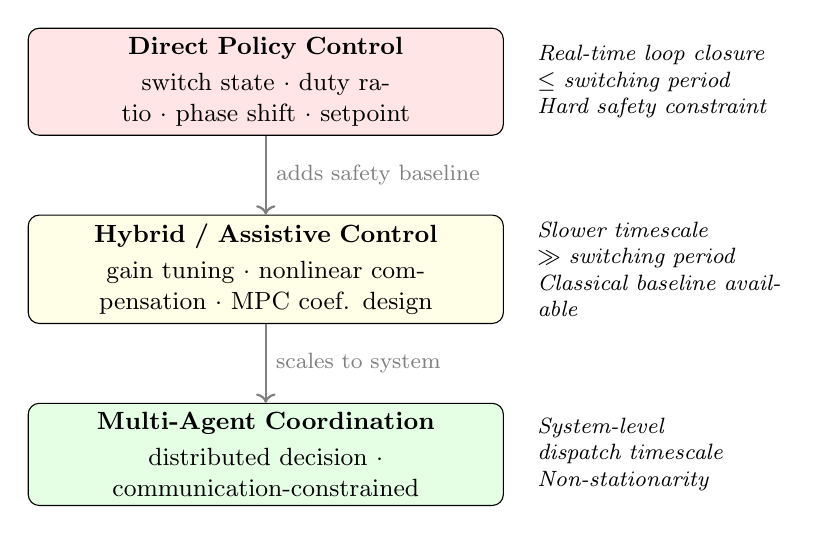
\begin{tikzpicture}[
  node distance=1.0cm,
  box/.style={draw, rounded corners, fill=blue!5, text width=5.8cm, align=center, minimum height=1.1cm, font=\small},
  labelbox/.style={text width=3.2cm, align=left, font=\footnotesize\itshape}
]
\node[box, fill=red!10] (direct) {\textbf{Direct Policy Control}\\[2pt] switch state $\cdot$ duty ratio $\cdot$ phase shift $\cdot$ setpoint};
\node[box, fill=yellow!10, below=of direct] (hybrid) {\textbf{Hybrid / Assistive Control}\\[2pt] gain tuning $\cdot$ nonlinear compensation $\cdot$ MPC coef. design};
\node[box, fill=green!10, below=of hybrid] (coord) {\textbf{Multi-Agent Coordination}\\[2pt] distributed decision $\cdot$ communication-constrained};

\node[labelbox, right=0.3cm of direct] (l1) {Real-time loop closure\\$\leq$ switching period\\Hard safety constraint};
\node[labelbox, right=0.3cm of hybrid] (l2) {Slower timescale\\$\gg$ switching period\\Classical baseline available};
\node[labelbox, right=0.3cm of coord] (l3) {System-level\\dispatch timescale\\Non-stationarity};

\draw[->, thick, gray] (direct.south) -- (hybrid.north) node[midway, right, font=\footnotesize] {adds safety baseline};
\draw[->, thick, gray] (hybrid.south) -- (coord.north) node[midway, right, font=\footnotesize] {scales to system};
\end{tikzpicture}
\caption{Control-role stack showing where a learned agent enters the converter control loop. Direct policy control closes the real-time loop at the switching period and carries the strictest safety constraints. Hybrid/assistive control operates on a slower timescale with a classical baseline controller providing a safety fallback. Multi-agent coordination addresses distributed decision-making at the system level, where non-stationarity from other learning agents introduces additional complexity.}
\label{fig:control-role-stack}
\end{figure}

\subsection{Direct Policy Control}

In direct policy control, the DRL agent directly selects the physical control action that determines the converter's switching behavior.
The action can be a discrete switch state (on/off for each semiconductor device), a continuous duty ratio, a phase-shift angle (for DAB and other isolated topologies), a modulation index, or a power/voltage setpoint that the inner control loop tracks without further learned intervention.

Direct switch control represents the most demanding interface: the agent must produce a gate-drive decision every switching period (typically 10--50~$\mu$s for hard-switched converters, and 100--500~$\mu$s for higher-power applications with lower switching frequencies).
The action space is discrete (on/off per switch), and the agent must respect hard constraints: no shoot-through (simultaneous conduction of complementary switches), no saturation, and no overcurrent during transient load steps.
Zandi et al.~\cite{zandi2023voltage} explored direct switch control for DC--DC converters using RL, demonstrating the feasibility of learned switching but also the challenge of guaranteeing constraint satisfaction at every time step.
Rajamallaiah et al.~\cite{rajamallaiah2024deep} applied a modified TD3-based DRL controller for voltage regulation of DC--DC buck converters feeding CPLs in DC microgrids, demonstrating that DRL can stabilize the negative-impedance instability of CPLs without requiring an explicit analytical model of the load dynamics.
Zandi and Poshtan~\cite{zandi2023voltage_quasi} extended this RL-based direct switching approach to quasi-Z-source converters under constant power load conditions, where the impedance-network dynamics introduce additional control challenges beyond those of conventional DC--DC topologies.
Qashqai et al.~\cite{qashqai2023model} applied model-free RL to direct switching control of a three-level neutral-point-clamped (NPC) converter, where the action must additionally balance the DC-link capacitor voltages.
More recently, Qashqai et al.~\cite{qashqai2025implementation} extended this approach to a 23-level hybrid packed U-cell (HPUC) converter using DQN, achieving model-free switching control with capacitor voltage balancing under noise and parameter variation---demonstrating scalability of direct switch-level DRL to higher-level-count topologies.
In modular multilevel converters (MMCs), Jung et al.~\cite{jung2022reinforcement} demonstrated RL-based modulation for balancing submodule capacitor voltages and equalizing thermal stress among semiconductor devices, extending learned control to higher-voltage, higher-cell-count topologies.
Gallardo et al.~\cite{gallardo2024reinforcement} further applied RL to MMC cybersecurity, training an RL-based detector to identify false data injection attacks on distributed MMC control architectures with hardware-in-the-loop validation.

Direct duty-ratio or phase-shift control relaxes the action-space constraint by operating on continuous variables rather than discrete switch states, making it compatible with policy-gradient and actor-critic algorithms designed for continuous control.
Ye et al.~\cite{ye2024deep} applied a DDPG-based controller for a single-inductor multiple-output (SIMO) DC--DC converter, where the agent outputs continuous duty ratios for each output channel---a multi-output control problem with cross-regulation that is difficult to solve with decoupled linear controllers.
Ye et al.~\cite{ye2025soft} later extended this approach to a single-inductor dual-output (SIDO) converter using an SAC-based controller, demonstrating strong robustness to input voltage, reference, and load variations.
Tang et al.~\cite{tang2020reinforcement,tang2021deep,tang2022deep,tang2021artificial} published a series of studies applying RL (including tabular Q-learning, DDPG, and TD3) to efficiency optimization and reactive power minimization of DAB converters through triple-phase-shift (TPS) modulation, where the agent selects the three phase-shift angles that minimize current stress, reactive power, or maximize efficiency under varying load and voltage conditions.
In these studies, the DRL agent acts as a direct modulation optimizer: it selects the phase-shift parameters that determine the converter's instantaneous operating point, replacing a lookup table or a model-based optimization routine.
Wu et al.~\cite{wu2021innovative} similarly applied DDPG to DAB converter control, focusing on DC bus voltage stabilization under load disturbances.
Feng et al.~\cite{feng2025six} extended DAB modulation optimization to six control degrees of freedom using DDPG, jointly optimizing switching frequency, phase shifts, and duty cycles via frequency-domain analysis to minimize RMS current and extend zero-voltage-switching range---experimentally validated on a hardware prototype.
Beyond modulation optimization, Gheisarnejad and Khooban~\cite{gheisarnejad2020iot} demonstrated a DRL-tuned active disturbance rejection control (ADRC) scheme for a DC--DC converter deployed on an IoT-enabled platform---a hybrid architecture where the DRL agent adjusts ADRC parameters online---providing early evidence that learned controllers can meet real-time embedded constraints, a finding whose deployment significance is discussed further in Section~\ref{sec:sim-to-real}.

\subsection{Hybrid and Assistive Control}

In hybrid control, the DRL agent does not directly select the switching action.
Instead, it tunes, compensates, or supervises a classical controller that retains real-time loop closure.
This architecture is more conservative but also more practical for near-term deployment: the classical controller provides a safety baseline (a known-stable controller that can operate alone), and the DRL component improves performance in operating regimes where the classical design is suboptimal.

Several distinct hybrid roles have emerged in the verified literature:

\textbf{Controller-gain and coefficient tuning.}
Gheisarnejad Chirani et al.~\cite{gheisarnejad2022reducing} used PPO with actor-critic networks to design the key coefficients of a model-free sliding-mode controller (MFSMC) for stabilizing a DC microgrid with parallel boost converters feeding CPLs.
The sliding-mode structure enforces a robustness baseline; the PPO-tuned coefficients improve the tradeoff between chattering and convergence speed.
Khooban~\cite{khooban2022smartenance} embedded DDPG-trained actor-critic networks in a non-integer MPC framework for DC--DC converters onboard a full-electric ferry, where the DRL agent designs the MPC coefficients.
In both cases, the DRL component operates on a slower timescale than the underlying controller: it updates coefficients periodically rather than at the switching frequency.

\textbf{Nonlinear compensation.}
Meng et al.~\cite{meng2022novel} proposed a TD3-assisted compensation strategy for a DAB converter feeding CPLs.
The base controller consists of a nonlinear disturbance observer and a backstepping controller that stabilizes the output voltage.
The TD3-trained agent provides an adaptive compensation signal that counteracts the destabilizing effect of the CPL's negative incremental impedance---a nonlinear phenomenon that is difficult to compensate with a fixed-gain observer.
The DRL component thus extends the operating envelope of an already-stable controller rather than replacing it.

\textbf{Adaptive gain learning.}
Hajihosseini et al.~\cite{hajihosseini2020dc} demonstrated a DRL-assisted ultra-local-model (ULM) feedback control architecture for a DC--DC buck-boost converter.
The learned component adapts the ULM feedback gains online, using an actor-critic DRL structure implemented on a dSPACE MicroLabBox real-time testbed.
This is one of the few verified examples of \emph{online DRL adaptation} (not merely offline-trained inference) on a real-time controller platform, making it significant deployment evidence despite the absence of a named sub-algorithm label.

\textbf{MPC parameter tuning.}
Several studies explore DRL for tuning MPC parameters that are otherwise heuristically selected.
Cui et al.~\cite{cui2023adaptive} used DRL to adapt the prediction horizon of a generalized predictive controller for DC--DC converters, replacing the fixed-horizon design with a policy that selects the horizon based on the operating condition.
He et al.~\cite{he2021weighting} applied RL to real-time updating of finite-control-set MPC (FCS-MPC) weighting factors, a task that is classically performed through offline trial-and-error.
Vazquez et al.~\cite{vazquez2022artificial} extended this concept using a supervised artificial neural network (ANN) for real-time FCS-MPC weighting factor tuning, implemented on low-cost control hardware---demonstrating a practical deployment path for learning-based (non-RL) MPC adaptation.
Liu et al.~\cite{liu2023reinforcement} further proposed an event-triggered FCS-MPC scheme where RL not only tunes the weighting factors but also determines when the MPC optimization should be invoked, reducing the average computational load.
Liu et al.~\cite{liu2024predictive} later extended RL-MPC integration to online learning: an actor-critic architecture learns a strategic utility function and derives control actions online for voltage source inverters, with Lyapunov analysis guaranteeing uniformly ultimate boundedness of all closed-loop signals.
Extending this direction to three-phase NPC converters, Liu et al.~\cite{liu2024event} combined event-driven protocols with online neural-network approximators for model-free predictive control, demonstrating that RL can simultaneously reduce switching frequency and handle parametric uncertainties.
Liu et al.~\cite{liu2024learning} further addressed cybersecurity by incorporating RL-based resilient FCS-MPC that maintains control integrity under actuator false data injection attacks.

The hybrid-control category is important for two reasons beyond accurate classification.
First, it reveals that a substantial portion of the ``DRL for converter control'' literature is, in computing terms, DRL for \emph{controller adaptation} rather than for \emph{controller replacement}.
Second, hybrid architectures offer a natural path for incremental deployment: the classical controller guarantees a minimum level of safety and performance, while the DRL module improves performance in regimes where it has been trained and validated.

\subsection{Multi-Agent Coordination}

In converter-dense systems---modular converters, input-series-output-parallel (ISOP) or input-series-output-series (ISOS) DAB systems, DC solid-state transformers, and DC microgrids with multiple converter interfaces---the control problem shifts from single-loop regulation to \emph{distributed decision-making under communication constraints}.
Each agent may control one converter module, and the agents must coordinate to achieve system-level objectives (voltage regulation, current sharing, power balance) while respecting local constraints and tolerating communication delay, packet loss, or partial observability.

This category is treated in depth in Section~\ref{sec:coordination}.
At this stage, it is sufficient to note that multi-agent control is not merely a scaled version of single-agent control: it introduces non-stationarity (each agent's environment changes as other agents update their policies), credit-assignment across agents, and communication-efficiency tradeoffs that are absent from single-converter problems.

Table~\ref{tab:deployment-taxonomy} (presented in Section~\ref{sec:taxonomy}) provides the complete control-role axis along with the associated action interfaces and the significance of each classification for CSUR synthesis.

%=====================================================================
\section{Algorithmic Families Through Control Interfaces}
\label{sec:algorithms}
%=====================================================================

A computing survey of DRL for converter control must discuss algorithms, but it must discuss them through the lens of their \emph{compatibility with the control interface} rather than through a generic tutorial on RL algorithm mechanics.
The question is not ``how does DQN work'' but rather ``why would one choose DQN, DDPG, TD3, SAC, or PPO for a specific control role, action space, sample budget, and safety requirement.''
This section therefore compares the major algorithm families by their action-interface compatibility, sample efficiency, stability behavior, and real-time control-loop constraints.
Algorithm-distribution statistics are not presented because the source-level verification required for such statistics is, at this stage, incomplete for the majority of candidate papers in the evidence table (Section~\ref{sec:synthesis}).
For a comprehensive treatment of RL foundations, the reader is referred to Sutton and Barto~\cite{sutton2018reinforcement}.

\subsection{Value-Based Methods: Discrete Actions, Off-Policy Learning}

Value-based methods---DQN~\cite{mnih2015human} and its extensions (Double DQN~\cite{van2016deep}, Dueling DQN, prioritized experience replay)---learn an action-value function $Q(s,a)$ and select actions by $\epsilon$-greedy or Boltzmann exploration over the estimated Q-values.
Their primary strength for converter control is off-policy learning with a replay buffer, which improves sample efficiency by reusing past experience.
Their primary limitation is the discrete action space: DQN natively outputs a Q-value for each discrete action, which maps naturally to discrete switch-state selection but poorly to continuous duty-ratio or phase-shift optimization.

In the converter-control literature, DQN and its variants have been applied to problems with naturally discrete or discretized action spaces, such as switch-state selection in DC--DC converters~\cite{zandi2023voltage}.
In the adjacent domain of electric motor drives, Schenke and Wallscheid~\cite{schenke2021deep} demonstrated a DQN-based direct torque controller for permanent magnet synchronous motors, illustrating how discrete-action RL can be applied to power-electronic actuation problems.
An early precursor explored tabular Q-learning (a non-deep value-based method) for modulation-mode selection in DAB converters~\cite{tang2020reinforcement}, illustrating the historical progression from look-up-table representations to function-approximation methods before DQN entered this application domain.
In adjacent energy-conversion domains, Q-learning-based MPPT has been demonstrated for photovoltaic~\cite{chou2019maximum} (adjacent domain: PV MPPT, DQN-based) and wind-energy~\cite{wei2015reinforcement} (adjacent domain: wind-energy MPPT, tabular Q-learning); RL-based control has also been explored for DC-AC converters~\cite{nicola2022comparative} (adjacent domain: DC-AC converter with robust passivity-based control) and DAB-based EV chargers~\cite{mahazabeen2022performance} (adjacent domain: EV charging with RL-tuned PI); Ahmadian et al.~\cite{ahmadian2024empowering} later applied TD3 to bidirectional VSI control for EV on-board chargers, enabling four-quadrant active and reactive power control across V2G and G2V modes; these are noted here for algorithmic context but are not counted in the converter-control evidence base.
However, discretizing a continuous variable (e.g., a duty ratio from 0 to 1 into 100 bins) introduces a tradeoff between resolution and action-space dimensionality: fine discretization produces many actions, slowing learning, while coarse discretization limits control precision and may introduce limit cycles.

An important methodological caution: the prior broad-scope review contained multiple classification errors in which DQN, Double DQN, and Q-learning labels were confused or interchanged.
A source-level cross-check of the prior review's algorithm assignments documented cases where a paper using DQN was classified under Q-learning, and vice versa.
Paper A avoids repeating these errors by requiring source-level algorithm verification before any source enters a named-algorithm figure or statistic.

\subsection{Policy-Gradient and Actor-Critic Methods: Continuous Actions}

For continuous action spaces---duty ratios, phase-shift angles, modulation indices, and controller coefficients---policy-gradient and actor-critic methods are the natural choice.
These algorithms parameterize a policy $\pi_\theta(a|s)$ that directly outputs continuous actions, typically as the mean and variance of a Gaussian distribution.

\textbf{DDPG} (Deep Deterministic Policy Gradient)~\cite{lillicrap2016continuous} extends the deterministic policy gradient (DPG) algorithm~\cite{silver2014deterministic} by combining a deterministic policy (actor) with a Q-function (critic) trained via off-policy experience replay and target networks.
It has been applied to continuous duty-ratio control in SIMO DC--DC converters~\cite{ye2024deep}, coefficient design for non-integer MPC~\cite{khooban2022smartenance}, and DAB phase-shift optimization~\cite{tang2021deep}.
Balouji et al.~\cite{balouji2025deep} applied DDPG-based deep reinforcement learning to provide adaptive virtual inertia for grid-supporting inverters in networks with electric arc furnaces, demonstrating that policy-gradient methods can learn to mitigate severe voltage flicker caused by highly nonlinear and rapidly varying industrial loads.
DDPG's deterministic policy is computationally efficient at inference time (a single forward pass through the actor network), but its exploration relies on added noise, which can produce unsafe actions during training unless constrained.

\textbf{TD3} (Twin Delayed Deep Deterministic Policy Gradient)~\cite{fujimoto2018addressing} addresses DDPG's overestimation bias and sensitivity to hyperparameters through three modifications: twin Q-networks (taking the minimum for conservative estimates), delayed policy updates, and target policy smoothing.
In the verified converter-control evidence, Meng et al.~\cite{meng2022novel} used TD3 for nonlinear compensation in a DAB backstepping controller, where the conservative Q-estimation may help avoid overconfident compensation signals that could drive the system toward instability.

\textbf{SAC} (Soft Actor-Critic)~\cite{haarnoja2018soft} adds an entropy-regularization term to the objective, encouraging exploration and producing stochastic policies that can be more robust to unmodeled dynamics.
SAC's maximum-entropy framework is theoretically appealing for converter control because it naturally resists premature convergence to narrow operating policies that fail under distribution shift.
However, the verified evidence for SAC in converter control is, at present, limited: Fathollahidehkordi et al.~\cite{fathollahi2023robust} is conditionally flagged as SAC-based robust parameter tuning, but the classification is not yet source-verified.

\textbf{PPO} (Proximal Policy Optimization)~\cite{schulman2017proximal} is an on-policy method that builds on trust-region policy optimization (TRPO)~\cite{schulman2015trust} and constrains policy updates to a trust region, improving training stability at the cost of lower sample efficiency (since on-policy data cannot be reused from a replay buffer).
In the verified evidence, Gheisarnejad Chirani et al.~\cite{gheisarnejad2022reducing} used PPO for MFSMC coefficient tuning with OPAL-RT HIL validation.
PPO's stability is attractive for safety-critical tuning tasks, but its lower sample efficiency can be a limitation when each episode requires running a detailed circuit simulation or a physical experiment.

\textbf{Actor-critic with ULM adaptation.}
Hajihosseini et al.~\cite{hajihosseini2020dc} demonstrated a DRL architecture that uses actor-critic learning for online adaptation of ULM feedback gains, implemented on a dSPACE MicroLabBox real-time platform.
The architecture is significant because it shows that actor-critic DRL can run in a real-time control loop without being instantiated as a specific named variant (DDPG, TD3, SAC, PPO), provided the network architecture and learning rule are designed for the target embedded platform.

\subsection{Model-Informed and Model-Based RL}

Model-based RL learns or uses a dynamics model to plan actions, potentially improving sample efficiency by orders of magnitude compared to model-free methods~\cite{moerland2023model}.
For power electronic converters, the dynamics are partially known: the circuit equations (averaged or switched) provide a nominal model, but parasitic elements, thermal effects, aging, and load behavior introduce uncertainty.
Model-informed RL occupies the middle ground: it uses the known circuit structure to accelerate learning or constrain the policy, without requiring a perfect model.

Huangfu et al.~\cite{huangfu2022learning} proposed a learning-based large-signal stabilization method for DC--DC boost converters feeding CPLs, where the learned policy is informed by the converter's large-signal model.
Wu et al.~\cite{wu2025deep} proposed a Lyapunov-constrained DDPG framework for deep synchronization control of grid-forming converters, where a learned deep dynamics model is combined with Lyapunov stability constraints to guarantee asymptotic convergence of the synchronization error while optimizing transient performance.
Qie et al.~\cite{qie2022new} developed a robust integral RL controller for interleaved DC--DC boost converters, where the integral action provides steady-state error elimination while the RL component adapts the control law to disturbances and parameter variations.
These methods demonstrate that incorporating power-electronics domain knowledge into the RL formulation---through model-based initialization, structured state representations, or constrained action spaces---can reduce the training burden and improve safety compared to purely model-free approaches.
This principle is consistent with sample-efficient actor-critic methods developed in the broader RL literature, such as ACER~\cite{wang2016sample}, which combine experience replay with off-policy corrections to improve data efficiency, and transfer learning frameworks that allow policies trained on one task or domain to accelerate learning on related tasks~\cite{lazaric2012transfer,parisotto2016actor}.

\subsection{Multi-Agent RL}

For coordination problems (Section~\ref{sec:coordination}), multi-agent RL (MARL) algorithms extend the single-agent frameworks to multiple interacting learners.
MADDPG (Multi-Agent DDPG)~\cite{lowe2017multi} extends DDPG with centralized critics that access all agents' observations and actions during training, while actors use only local observations during execution---the centralized-training-decentralized-execution (CTDE) paradigm.
Zeng et al.~\cite{zeng2022autonomous,zeng2022multiagent} applied multi-agent DRL to ISOP-DAB systems, where agents coordinate input-voltage sharing and output-current sharing among series-connected DAB modules.
MAPPO~\cite{yu2022surprising} extends PPO to the multi-agent setting with similar CTDE structure, and has been shown to be surprisingly effective on cooperative multi-agent benchmarks.

The key computational distinction between single-agent and multi-agent RL for converter control is not the algorithm mechanics but the introduction of \emph{non-stationarity} and \emph{communication constraints}.
When multiple learned agents control interconnected converters, each agent's environment includes the actions of other learning agents, violating the Markov assumption that underlies single-agent RL convergence theory.
This topic is discussed further in Section~\ref{sec:coordination}.

%=====================================================================
\section{Deployment-Centered Taxonomy}
\label{sec:taxonomy}
%=====================================================================

This taxonomy organizes learned converter control along six computing-relevant axes rather than by converter topology or algorithm family.
This taxonomy, summarized in Table~\ref{tab:deployment-taxonomy}, is the organizing contract for the rest of the manuscript.
Each source is first assigned a control role and action interface, then checked against safety, deployment, computation, and coordination evidence.
Algorithm labels such as DQN, TD3, PPO, SAC, DDPG, MADDPG, or MAPPO are recorded only after this functional placement is complete.

\begin{table*}[t]
\caption{Deployment-centered taxonomy for DRL-based real-time converter control. The taxonomy is designed to classify the computational role of the learned component before counting algorithm names.}
\label{tab:deployment-taxonomy}
\begin{tabular}{p{0.17\textwidth}p{0.32\textwidth}p{0.42\textwidth}}
\toprule
Axis & Classification labels & Why the axis matters for CSUR synthesis \\
\midrule
Control role & Direct policy control; setpoint or duty-ratio control; modulation optimization; nonlinear-control compensation; controller-gain or coefficient tuning; supervisory coordination & Separates learned controllers that close the real-time loop from DRL modules that tune or assist an existing controller. This prevents hybrid MPC, sliding-mode, and backstepping designs from being counted as direct learned switching control. \\
Action interface & Discrete switch action; continuous duty ratio; phase-shift or modulation parameter; controller coefficient; reference or power-sharing command & Links algorithm families to physical actuation constraints, sampling frequency, safety envelope, and embedded implementation requirements. \\
Safety mechanism & Reward penalty; constrained action set; robust-control wrapper; Lyapunov/barrier certificate; runtime shield; fallback controller; post-training stress test & Distinguishes empirical safety from mechanisms that can support stability, certification, and deployment claims. \\
Deployment maturity & Simulation only; real-time digital simulation; controller-HIL; power-HIL; embedded prototype; field-relevant deployment & Keeps proof-of-concept evidence separate from hardware-ready evidence and avoids unsupported adoption timelines. \\
Computational stage & Offline training; online inference; online adaptation; memory footprint; communication overhead; retraining or transfer cost & Forces computational-efficiency claims to specify which cost is being measured rather than treating training and deployment cost as one quantity. \\
Coordination scope & Single converter; converter module cluster; DAB/SST sharing; DC microgrid; converter-dense CPS; multi-energy network & Identifies when the computing problem shifts from single-loop control to distributed decision-making under communication, observability, and scalability limits. \\
\bottomrule
\end{tabular}
\end{table*}

The rationale for replacing a converter-type taxonomy with a deployment-centered one is both methodological and practical.
Methodologically, a converter-type organization (``DRL for buck converters,'' ``DRL for boost converters,'' ``DRL for DAB converters'') groups papers that share a plant but may differ in every computing dimension: one buck-converter paper may use DQN for direct switch control in simulation, while another may use PPO to tune a PID controller on an embedded DSP.
Grouping them by ``buck converter'' obscures the computing differences that determine deployment feasibility.
Practically, the prior broad-scope review's converter-type classification was directly criticized by reviewers for lumping together direct control, hybrid control, and unrelated maintenance papers under the same topology heading.

Each axis of the deployment taxonomy is now examined in its own section (Sections~\ref{sec:safety}--\ref{sec:coordination}), with the evidence synthesis in Section~\ref{sec:synthesis} bringing the axes together.

%=====================================================================
\section{Safety, Stability, and Certification}
\label{sec:safety}
%=====================================================================

Safety and stability are deployment requirements, not future work.
A DRL-based converter controller that achieves 0.1\% voltage regulation in nominal simulation but issues a shoot-through command during a transient load step is not a deployable controller.
This section distinguishes six levels of safety assurance, from weakest to strongest, and provides verified examples at each level.
It also specifies conditions under which DRL should \emph{not} be used, establishing the negative guidance that is necessary for credibility with both computing-systems and power-electronics reviewers.

\begin{figure}[t]
\centering
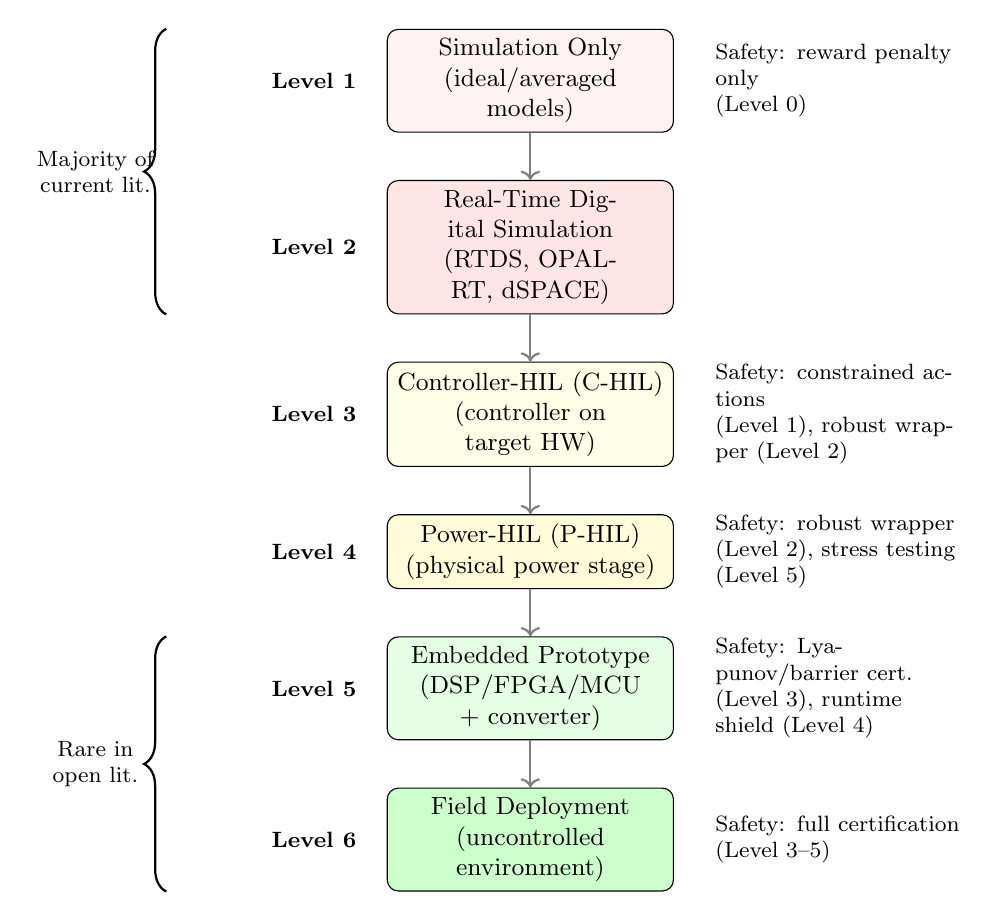
\begin{tikzpicture}[
  node distance=0.6cm,
  ladder/.style={draw, rounded corners, fill=blue!5, text width=3.4cm, align=center, minimum height=0.8cm, font=\small},
  safety/.style={text width=3.2cm, align=left, font=\footnotesize},
  level/.style={font=\footnotesize\bfseries, text width=1.2cm, align=center}
]
% Left column: ladder steps
\node[ladder, fill=red!5] (L1) {Simulation Only\\(ideal/averaged models)};
\node[ladder, fill=red!10, below=of L1] (L2) {Real-Time Digital Simulation\\(RTDS, OPAL-RT, dSPACE)};
\node[ladder, fill=yellow!10, below=of L2] (L3) {Controller-HIL (C-HIL)\\(controller on target HW)};
\node[ladder, fill=yellow!15, below=of L3] (L4) {Power-HIL (P-HIL)\\(physical power stage)};
\node[ladder, fill=green!10, below=of L4] (L5) {Embedded Prototype\\(DSP/FPGA/MCU + converter)};
\node[ladder, fill=green!20, below=of L5] (L6) {Field Deployment\\(uncontrolled environment)};

% Right column: safety levels
\node[safety, right=0.4cm of L1] (S1) {Safety: reward penalty only\\(Level~0)};
\node[safety, right=0.4cm of L2] (S2) {};
\node[safety, right=0.4cm of L3] (S3) {Safety: constrained actions\\(Level~1), robust wrapper (Level~2)};
\node[safety, right=0.4cm of L4] (S4) {Safety: robust wrapper\\(Level~2), stress testing (Level~5)};
\node[safety, right=0.4cm of L5] (S5) {Safety: Lyapunov/barrier cert.\\(Level~3), runtime shield (Level~4)};
\node[safety, right=0.4cm of L6] (S6) {Safety: full certification\\(Level~3--5)};

% Arrows between ladder steps
\draw[->, thick, gray] (L1.south) -- (L2.north);
\draw[->, thick, gray] (L2.south) -- (L3.north);
\draw[->, thick, gray] (L3.south) -- (L4.north);
\draw[->, thick, gray] (L4.south) -- (L5.north);
\draw[->, thick, gray] (L5.south) -- (L6.north);

% Level labels on left
\node[level, left=0.2cm of L1] {Level 1};
\node[level, left=0.2cm of L2] {Level 2};
\node[level, left=0.2cm of L3] {Level 3};
\node[level, left=0.2cm of L4] {Level 4};
\node[level, left=0.2cm of L5] {Level 5};
\node[level, left=0.2cm of L6] {Level 6};

% Majority marker
\draw[decorate,decoration={brace,amplitude=8pt,mirror}, thick]
  ([xshift=-2.8cm]L1.north west) -- ([xshift=-2.8cm]L2.south west)
  node[midway, xshift=-0.9cm, font=\footnotesize, align=center] {Majority of\\current lit.};

\draw[decorate,decoration={brace,amplitude=8pt,mirror}, thick]
  ([xshift=-2.8cm]L5.north west) -- ([xshift=-2.8cm]L6.south west)
  node[midway, xshift=-0.9cm, font=\footnotesize, align=center] {Rare in\\open lit.};
\end{tikzpicture}
\caption{Safety and deployment ladder: six validation maturity levels with corresponding safety assurance levels. The majority of the current literature clusters at Levels~1--2 (simulation only and real-time digital simulation). Levels~3--4 (C-HIL and P-HIL) are demonstrated by a small number of verified sources. Levels~5--6 (embedded prototype and field deployment) remain rare in the open literature. Each step up the ladder requires additional safety mechanisms beyond reward penalties.}
\label{fig:safety-deployment-ladder}
\end{figure}

\subsection{Level 0: Reward-Only Penalty}

The most common safety mechanism in the DRL-for-converter-control literature is a penalty term added to the reward function: a large negative reward when the output voltage exceeds a bound, the inductor current saturates, or a switching stress limit is violated.
Reward penalties discourage unsafe behavior during training but provide no guarantee during deployment.
An untrained or partially trained policy can still produce unsafe actions, and a trained policy can fail when the operating condition differs from the training distribution.
Jiang et al.~\cite{jiang2023stability} addressed this limitation explicitly by framing stability as a multi-objective optimization problem, where stability-oriented terms in the reward are combined with control-performance terms, but they acknowledged that reward shaping alone does not provide a stability guarantee.

Paper~A's position is that \textbf{reward-only penalty is not a sufficient safety mechanism for any deployment claim}.
It is acceptable for simulation-only proof-of-concept studies, but any paper that claims ``safe operation,'' ``robustness,'' or ``reliability'' based solely on reward engineering should be treated as Level~0 safety evidence.
The broader safe-RL literature has long recognized that reward shaping alone cannot guarantee safety during exploration or deployment~\cite{garcia2015comprehensive,moldovan2012safe}.

\subsection{Level 1: Constrained Action Set}

A stronger mechanism constrains the agent's action space to exclude known-unsafe actions.
For a buck converter, this means prohibiting duty ratios that would cause inductor saturation; for a DAB converter, prohibiting phase-shift combinations that cause DC bias in the transformer.
The constraint can be enforced by projecting the policy's output onto the safe action set (action clipping or projection) or by masking unsafe actions before the selection step (in discrete-action methods).

Constrained action sets are a natural application of power-electronics domain knowledge: the safe operating area of a converter is well-understood from circuit theory, and encoding it as action bounds provides a hard guarantee that the learned policy cannot violate steady-state constraints.
However, it does not protect against unsafe \emph{sequences} of actions---for example, a sequence of individually-safe duty-ratio steps that collectively drive the system into a large-signal instability.

\subsection{Level 2: Robust-Control Wrapper}

A robust-control wrapper embeds the learned policy inside a classical robust controller, such that the classical controller guarantees bounded-input-bounded-output (BIBO) stability or a specified $\mathcal{H}_\infty$ performance level, while the DRL component improves performance within that stable envelope.
This approach is exemplified by the PPO-assisted MFSMC architecture of Gheisarnejad Chirani et al.~\cite{gheisarnejad2022reducing}: the sliding-mode controller provides a stable baseline, and the PPO-tuned coefficients improve the tradeoff between chattering and convergence speed without breaking the sliding-mode stability conditions.

Similarly, Meng et al.~\cite{meng2022novel} combined a TD3-trained compensation signal with a backstepping controller stabilized by a nonlinear disturbance observer.
Zhou et al.~\cite{zhou2023drl} applied an SAC-based parameter self-configuration mechanism for nonsmooth composite control in DC microgrids with CPLs, where the DRL agent tunes a fractional-order robustness factor to balance disturbance rejection against chattering.
The backstepping controller alone is provably stable (under the standard backstepping Lyapunov argument), and the TD3 compensation signal is additive---it does not replace the stabilizing feedback law.
In the event of DRL failure, the base controller continues to operate, albeit with reduced performance.

The robust-control-wrapper category is significant because it represents a pragmatic middle ground between ``pure DRL with reward penalty'' and ``formal DRL safety certification.''
For many converter applications, the robust wrapper is the most practical path to near-term deployment: it leverages existing stability theory while allowing DRL to extend the performance envelope.

\subsection{Level 3: Lyapunov and Barrier Certificates}

The strongest current safety mechanisms---those that can support formal stability or safety claims---integrate Lyapunov functions or control barrier functions (CBFs) into the DRL training or execution process.
A Lyapunov-based approach trains the critic network to approximate a Lyapunov function for the closed-loop system, and the policy is constrained to actions that decrease the Lyapunov function (or keep it within a safe sublevel set).
A CBF-based approach defines a barrier function that is positive in the safe set and approaches zero at the boundary; the policy is constrained to actions that keep the barrier function above a threshold, guaranteeing forward invariance of the safe set.

In the converter-control literature, Level~3 mechanisms remain largely aspirational.
The existing verified evidence does not contain a complete Lyapunov-constrained or CBF-constrained DRL controller for a power electronic converter with hardware validation.
However, the theoretical machinery is well-developed in the broader safe-RL literature: Chow et al.~\cite{chow2018lyapunov} proposed a Lyapunov-based approach that constrains the policy to actions that decrease a learned Lyapunov function; Ames et al.~\cite{ames2019control} provided a comprehensive treatment of control barrier functions for safety-critical control; and Fisac et al.~\cite{fisac2019general} developed a reachability-based safety framework for learning-based control that guarantees constraint satisfaction while minimally interfering with the learning process.
Initial steps toward converter-specific barrier design have been taken in simulation studies, but the integration of these theoretical tools with the microsecond-timescale and hard-switching constraints of power electronic converters remains an open problem.
This gap is identified as a high-priority research direction (Section~\ref{sec:agenda}, Row~1 of Table~\ref{tab:research-agenda}).

\subsection{Level 4: Runtime Shielding and Fallback Control}

A runtime shield monitors the policy's output at each time step and overrides it with a safe fallback action if the proposed action would violate a safety constraint.
The simplest shield is a saturation block that clips the action to safe bounds (Level~1).
A more sophisticated shield simulates the proposed action forward by one or more time steps (using a simplified plant model) and checks whether any state variable would exit the safe region.
If the shield predicts a violation, it substitutes a fallback action from a safe baseline controller (e.g., a PI controller or a lookup table).

Weber et al.~\cite{weber2023steady} addressed a related problem: steady-state error compensation for RL-based control of power electronic systems.
Their method uses a correction term to eliminate the steady-state error that RL controllers often exhibit, effectively acting as a post-processing shield that ensures the steady-state specification is met.
Full runtime shielding with forward-simulation-based action filtering has not yet been demonstrated in the verified converter-control literature, but it is a natural extension of existing work on action projection and fallback control.
In the broader AI literature, Alshiekh et al.~\cite{alshiekh2018safe} demonstrated the shielding paradigm: a reactive system (the shield) monitors the RL agent's output and overrides any action that would violate a temporal-logic safety specification, while otherwise leaving the agent free to optimize performance.

In the power converter domain, Wan et al.~\cite{wan2024safety} proposed a safety-enhanced self-learning framework that enables safe online RL on a physical two-level voltage source converter, addressing the core challenge that standard RL exploration can produce unsafe switching actions on real hardware.
Their method demonstrates that online learning on physical converters is feasible when the exploration process is constrained to a verified safe region.

\subsection{Level 5: Post-Training Validation and Stress Testing}

The final safety level applies after training: the learned policy is subjected to a systematic stress-test battery that includes worst-case load steps, input-voltage sags and swells, component parameter drift (inductance, capacitance, ESR), sensor noise injection, communication delays, and EMI-induced measurement errors.
Post-training validation does not guarantee safety---it can only demonstrate safety for the tested scenarios---but it is an essential prerequisite for any deployment claim.

The current literature rarely reports systematic stress testing.
Most papers report a small number of nominal and perturbed operating conditions, selected to demonstrate the controller's advantage rather than to probe its failure modes.
Paper~A therefore includes post-training stress testing as a required reporting item in the reproducibility checklist (Table~\ref{tab:reproducibility-checklist}, row~4).

\subsection{When Not to Use DRL}

DRL is not a universal replacement for power-electronics control theory.
It adds value when the control problem involves high-dimensional observations, nonlinear or time-varying dynamics, multi-objective tradeoffs, or distributed decision-making where hand-designed policies are brittle.
It adds risk when the operating envelope is narrow, safety constraints are hard, the latency budget is tight (sub-10~$\mu$s), and an accurate low-order model exists.

Concretely, if a buck converter operates at a fixed input voltage, a fixed load, and a fixed switching frequency, a well-tuned Type-III compensator or PI controller will achieve excellent regulation with zero training cost, zero inference latency (a few multiply-add operations in fixed-point arithmetic), and formal stability guarantees from classical control theory.
Introducing DRL in this setting adds complexity without adding value.

DRL becomes more compelling when:
\begin{itemize}
  \item The load is a CPL, introducing nonlinear negative-impedance instability that challenges linear controllers~\cite{huangfu2022learning}.
  \item The converter operates across wide input-voltage and load ranges, where a single linear controller cannot be tuned for all operating points.
  \item Multiple objectives (efficiency, current stress, thermal balance, voltage regulation) must be traded off in real time~\cite{jiang2023stability}.
  \item The system includes multiple interacting converters with communication constraints, where centralized control is infeasible~\cite{zeng2022autonomous}.
\end{itemize}

This negative guidance---specifying when DRL is \emph{not} the right tool---is necessary for the survey's credibility.
It prevents the manuscript from being read as an uncritical endorsement of DRL for all converter-control problems and aligns with the principle that computing solutions should be chosen based on the problem's constraints, not on the solution's novelty.

%=====================================================================
\section{Sim-to-Real and Deployment Readiness}
\label{sec:sim-to-real}
%=====================================================================

A DRL controller that performs well in an idealized Simulink or PLECS simulation has not demonstrated deployment readiness.
The gap between simulation and hardware is well-known in robotics and autonomous driving~\cite{zhao2020sim}, but it takes a specific and severe form in power electronic converters: switching non-idealities (ringing, overshoot, dead-time distortion), electromagnetic interference (EMI), thermal drift of passive components, sensor quantization and delay, gate-driver propagation delay, and parasitic inductances and capacitances that are not modelled in an averaged or ideal-switch simulation.
This section defines a validation maturity ladder and analyzes the transfer challenges that must be addressed at each step.

\subsection{Validation Maturity Ladder}

Six levels of validation maturity are defined, from least to most deployment-relevant:

\begin{enumerate}
  \item \textbf{Simulation only.} The policy is trained and evaluated in an offline simulation environment (MATLAB/Simulink, PLECS, PSIM, or custom Python environment) with ideal or averaged switch models. The majority of the current literature falls into this category.
  \item \textbf{Real-time digital simulation.} The policy is evaluated on a real-time digital simulator (RTDS, OPAL-RT, or dSPACE) running a detailed switching model with fixed-step solvers at the target control frequency. This verifies that the policy's inference time is compatible with the real-time constraint but does not involve physical power hardware.
  \item \textbf{Controller-HIL (C-HIL).} The learned policy runs on the target embedded controller (DSP, FPGA, or MCU), and the controlled plant is simulated in real time on a separate real-time simulator. C-HIL validates the controller hardware, the inference latency, and the I/O interfaces under real-time conditions. Critically, C-HIL confirms that the embedded controller meets real-time timing constraints, but it does \emph{not} validate power-stage dynamics---some studies report ``HIL validation'' on the basis of C-HIL alone, which leaves the interaction with real power hardware (switching transients, thermal effects, EMI) untested. The distinction between C-HIL and P-HIL is therefore essential when assessing deployment-readiness claims.
  \item \textbf{Power-HIL (P-HIL).} The learned policy runs on the target embedded controller, and the plant includes physical power-stage hardware (the actual converter or a scaled prototype) with power amplifiers providing the source and load interfaces. P-HIL validates the full signal chain, including sensor noise, gate-driver dynamics, and EMI, under controlled but realistic power conditions.
  \item \textbf{Embedded prototype.} The learned policy runs on the final embedded hardware (DSP, FPGA, or MCU), controlling a physical converter prototype under laboratory conditions. This level requires the policy to be compiled, quantized, or synthesized for the target platform.
  \item \textbf{Field-relevant deployment.} The controller operates in a non-laboratory environment: an electric vehicle powertrain, a microgrid testbed, a maritime DC system, or an industrial converter. This level introduces uncontrolled environmental variation, long-duration reliability requirements, and human-operator interaction.
\end{enumerate}

The majority of verified evidence in Paper~A's bibliography is clustered at Levels~1 and~2.
Level~3 (C-HIL) is demonstrated by Gheisarnejad Chirani et al.~\cite{gheisarnejad2022reducing}, who used an OPAL-RT real-time simulator for HIL validation of the PPO-assisted MFSMC controller.
Level~4 (real-time embedded) is demonstrated by Hajihosseini et al.~\cite{hajihosseini2020dc}, who implemented the actor-critic DRL controller on a dSPACE MicroLabBox real-time testbed.
Levels~5 and~6 are rare in the open literature and represent a significant gap between the research frontier and deployment practice.

\subsection{Transfer Challenges}

Moving from one validation level to the next exposes specific computing challenges:

\textbf{Plant fidelity.}
An averaged switch model (Level~1) does not capture the switching ripple, dead-time distortion, or high-frequency ringing that a real-time switching model (Level~2) and physical hardware (Levels~4--6) introduce.
A policy trained on an averaged model may produce duty-ratio commands that, when applied to a real converter with dead-time, produce a different effective duty ratio and degrade regulation.

\textbf{Disturbance coverage.}
The training distribution of load steps, input-voltage variations, and parameter values determines the policy's generalization envelope.
If the training environment uses a narrow set of disturbance profiles, the policy may fail on unseen combinations.
Domain randomization---randomizing the load, input voltage, and component values during training---can improve robustness, but its effectiveness depends on the randomization range matching (or exceeding) the expected deployment range.
Domain randomization was originally developed in the robotics community for visual~\cite{tobin2017domain} and dynamics~\cite{peng2018sim} transfer, and has been extended with system identification to build more accurate simulators for sim-to-real transfer of agile locomotion~\cite{tan2018sim}.
Sim-to-real transfer with explicit discussion of randomization ranges has been demonstrated in the adjacent domain of electric motor control~\cite{book2021transferring}, and safe Bayesian optimization for data-driven power electronics control design has been validated on microgrid hardware~\cite{book2021safe}. More recently, Cui et al.~\cite{cui2023implementation} proposed a duty-ratio mapping methodology for transferring offline-trained DRL controllers to physical DC--DC buck converters, explicitly addressing the simulation-to-hardware mismatch through a calibrated output mapping rather than domain randomization alone. Lee et al.~\cite{lee2024reinforcement} tackled the complementary problem of DSP controller time delay by augmenting the training MDP with a virtual decision process that accounts for the delay between measurement and actuation, producing policies that transfer more robustly to real-time embedded platforms.
In the multi-module converter domain, Zeng et al.~\cite{zeng2025physics} developed a physics-informed deep transfer RL method that transfers knowledge from a simulation-trained ISOP-DAB system to a physical experimental system using minimal experimental data, while Zeng et al.~\cite{zeng2025multi} achieved a 96.4\% training reduction when transferring multi-objective grid-following controllers across converters with different system parameters.
In the grid-forming inverter domain, Oshnoei et al.~\cite{oshnoei2024grid} applied a soft actor-critic DRL algorithm for grid impedance shaping with HIL validation on a dSPACE platform---providing one of the few experimentally verified demonstrations that DRL can adaptively tune virtual impedance parameters to maintain stable operation under varying grid strength conditions.

\textbf{Sensor noise and quantization.}
The simulation state vector is typically noise-free and continuous.
A physical controller receives ADC readings with quantization error, offset, gain error, and noise.
If the policy has not been trained with sensor noise injection, it may amplify high-frequency noise through its action output, producing jittery switching that increases losses and EMI.

\textbf{Thermal drift and aging.}
Over time, the inductance of a power inductor can change by $\pm 20\%$ due to temperature and DC bias; the capacitance of electrolytic capacitors decreases with aging; the on-resistance of MOSFETs increases with temperature.
These slow parameter drifts shift the plant dynamics away from the training distribution.
Online adaptation (Section~\ref{sec:computation}) can track slow drift, but only if the adaptation mechanism is safe (does not explore unsafe actions during online updates) and computationally feasible.

\textbf{Dead-time and nonlinearities.}
In a physical half-bridge, dead-time insertion prevents shoot-through but introduces a nonlinear voltage distortion that depends on the load current direction and magnitude.
A simulation that neglects dead-time will produce optimistic regulation results that do not transfer to hardware.

Paper~A's position is that the validation maturity level must be explicitly stated and used to qualify all deployment-related claims.
A paper that reports simulation-only results cannot be used to support claims about ``real-time feasibility'' or ``hardware readiness,'' regardless of the simulation's fidelity.

%=====================================================================
\section{Computational Efficiency}
\label{sec:computation}
%=====================================================================

Computational cost in learned converter control is not a single number.
It comprises at least four distinct dimensions, each with its own measurement unit, bottleneck, and deployment implication.
Failing to separate these dimensions is one of the most common weaknesses in the current literature, where statements like ``the proposed method has low computational cost'' conflate a multi-GPU-week training budget with a 50~$\mu$s inference latency.
This section defines each dimension, surveys what the verified literature reports, and identifies what is missing.

\begin{figure}[t]
\centering
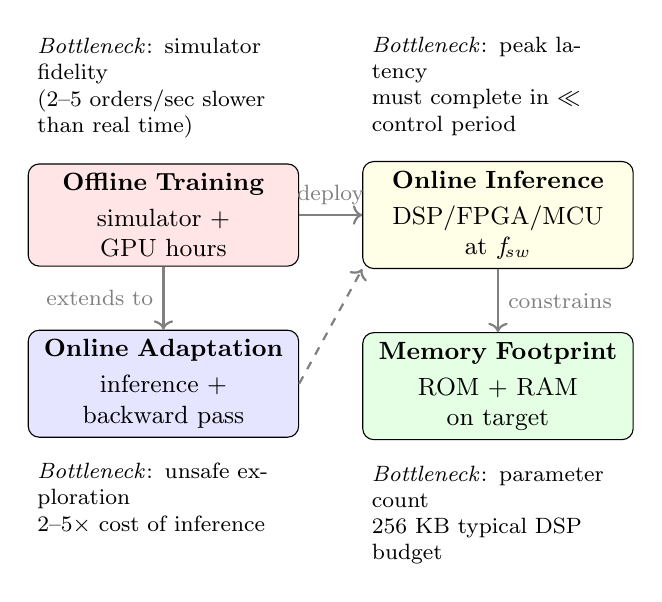
\begin{tikzpicture}[
  node distance=0.8cm,
  stage/.style={draw, rounded corners, fill=blue!5, text width=3.2cm, align=center, minimum height=1.0cm, font=\small},
  detail/.style={text width=3.2cm, align=left, font=\footnotesize}
]
\node[stage, fill=red!10] (train) {\textbf{Offline Training}\\[2pt] simulator + GPU hours};
\node[stage, fill=yellow!10, right=of train] (infer) {\textbf{Online Inference}\\[2pt] DSP/FPGA/MCU at $f_{\!sw}$};
\node[stage, fill=green!10, below=of infer] (mem) {\textbf{Memory Footprint}\\[2pt] ROM + RAM on target};
\node[stage, fill=blue!10, below=of train] (adapt) {\textbf{Online Adaptation}\\[2pt] inference + backward pass};

\node[detail, above=0.2cm of train] (d1) {\textit{Bottleneck}: simulator fidelity\\(2--5 orders/sec slower than real time)};
\node[detail, above=0.2cm of infer] (d2) {\textit{Bottleneck}: peak latency\\must complete in $\ll$ control period};
\node[detail, below=0.2cm of mem] (d3) {\textit{Bottleneck}: parameter count\\256~KB typical DSP budget};
\node[detail, below=0.2cm of adapt] (d4) {\textit{Bottleneck}: unsafe exploration\\$2$--$5\times$ cost of inference};

\draw[->, thick, gray] (train.east) -- (infer.west) node[midway, above, font=\footnotesize] {deploy};
\draw[->, thick, gray] (infer.south) -- (mem.north) node[midway, right, font=\footnotesize] {constrains};
\draw[->, thick, gray] (train.south) -- (adapt.north) node[midway, left, font=\footnotesize] {extends to};
\draw[->, thick, dashed, gray] (adapt.east) -- (infer.south west);
\end{tikzpicture}
\caption{Computational cost decomposition for DRL-based converter control. The four dimensions---offline training, online inference, memory footprint, and online adaptation---have distinct measurement units, bottlenecks, and deployment implications. Failing to separate them is a common weakness in current reporting. The dashed arrow from online adaptation back to inference indicates the feedback loop that makes online learning on a physical converter risky.}
\label{fig:computation-pipeline}
\end{figure}

\subsection{Offline Training Cost}

Offline training determines whether a method can be reproduced, adapted to a new converter topology, or retrained for a different operating envelope.
The cost includes the simulator's computational burden (e.g., a detailed switching Simulink model running at 100~ns resolution for 10$^6$ time steps per episode), the number of episodes or environment steps, the number of parallel environment instances, the GPU/CPU hardware used, and the wall-clock training time.

The verified literature rarely reports training cost in a form that enables reproduction or comparison.
Most papers state the number of episodes but omit the episode duration in environment steps, the simulation time step, the computational cost per simulation step, or the training hardware.
Without this information, a claim of ``sample-efficient learning'' is unverifiable: a method that converges in 500 episodes of 10~ms each (5~s of simulated experience) is not comparable to one that converges in 500 episodes of 100~ms each (50~s of simulated experience).

\subsection{Online Inference Latency}

Online inference latency determines whether the learned policy can execute within the control-loop period.
For a DC--DC converter switching at 100~kHz (10~$\mu$s period), the policy must compute its action in a fraction of that period---typically 1--5~$\mu$s for a DSP-based implementation, leaving the remaining time for ADC sampling, PWM update, and communication.
An actor network with two hidden layers of 128 neurons each requires approximately 20,000 multiply-accumulate operations per inference; whether this fits within the latency budget depends on the processor's clock speed, the availability of hardware multiply-accumulate units, and the precision (floating-point vs. fixed-point vs. quantized integer).

The verified literature contains few explicit latency measurements.
Hajihosseini et al.~\cite{hajihosseini2020dc} demonstrated real-time operation on a dSPACE MicroLabBox, which implies that the inference latency was within the control-loop period, but the exact latency value is not stated in accessible metadata.
Gheisarnejad Chirani et al.~\cite{gheisarnejad2022reducing} validated on OPAL-RT, which is a real-time simulator rather than an embedded controller, so the inference latency on the OPAL-RT's host processor may not represent the latency on a target DSP or MCU.
This gap---the absence of measured inference latency on target embedded hardware---is one of the most significant barriers to deployment claims.

\subsection{Memory Footprint}

Memory footprint determines whether the policy can be stored on the target embedded platform.
A DSP with 256~KB of RAM can store a policy network of roughly 64,000 parameters at 4 bytes per parameter (float32), plus buffers for the state, action, and intermediate activations.
Larger networks require external memory with higher access latency, or compression.

Policy compression techniques from the broader DRL literature---weight pruning, quantization (float32 to int8)~\cite{gholami2021survey}, knowledge distillation from a large teacher network to a small student network~\cite{hinton2015distilling}, and hardware-aware neural architecture search~\cite{cheng2018survey}---are directly applicable to converter control but have not been systematically explored in the verified evidence base.
The emerging TinyML paradigm~\cite{sanchez2020tinyml} provides a reference framework for deploying learned models on microcontroller-class devices with severe memory and energy constraints, but its techniques have not yet been applied to real-time converter control loops.
This review identifies hardware-aware policy design as a high-priority research direction (Section~\ref{sec:agenda}, Row~3 of Table~\ref{tab:research-agenda}).

\subsection{Online Adaptation and Retraining}

Online adaptation---updating the policy weights while the controller is running---introduces additional computational burden beyond inference.
An online learning step requires one forward pass (inference), one backward pass (gradient computation), and one weight update, which is typically $2$--$5\times$ more expensive than inference alone.
Moreover, online learning on a physical converter carries the risk of unsafe exploration: a weight update that degrades the policy can immediately produce unsafe actions.

Event-triggered inference and adaptation offer a partial solution: rather than evaluating the policy at every switching period, the controller evaluates it only when a significant change in the operating condition is detected (e.g., a load step exceeding a threshold or a voltage error exceeding a bound).
Between triggers, the controller holds the last action or falls back to a classical controller.
This approach reduces the average computational load and decouples the DRL inference period from the switching period, but it introduces a tradeoff between computational savings and response time.

The verified evidence for online adaptation in converter control is concentrated in the work of Hajihosseini et al.~\cite{hajihosseini2020dc}, where the actor-critic DRL controller adapted ULM feedback gains online using the dSPACE MicroLabBox platform.
This is treated as a Level~4 deployment-maturity example (real-time embedded) with the caveat that the specific online learning cost and the safety of online exploration are not fully documented in the accessible metadata.

%=====================================================================
\section{Coordination in Converter-Dense Systems}
\label{sec:coordination}
%=====================================================================

When multiple power electronic converters share a common DC bus, an AC grid connection, or a thermal management system, their controllers are no longer independent.
The coordination problem extends beyond single-loop regulation to distributed decision-making under communication constraints, partial observability, and non-stationarity arising from other agents' learning or adaptation.
This section frames multi-agent converter control as a deployment-architecture problem in cyber-physical computing, rather than as a scaled version of single-agent control.

\subsection{System Archetypes}

\textbf{Modular converters.}
Input-series-output-parallel (ISOP) and input-series-output-series (ISOS) DAB systems connect multiple converter modules to share voltage and current stresses, enabling higher-voltage and higher-power operation with lower-rated semiconductor devices.
The coordination task is to maintain balanced input-voltage sharing and output-current sharing among modules, despite parameter mismatches (transformer leakage inductance, capacitor ESR) and load variations.
Zeng et al.~\cite{zeng2022autonomous,zeng2022multiagent} applied multi-agent DRL to ISOP-DAB control, where each agent controls one DAB module and learns to coordinate its phase-shift adjustment with other agents to achieve autonomous input-voltage sharing and TPS modulation optimization.

\textbf{DC solid-state transformers (SST).}
An SST typically consists of a cascaded AC--DC front-end, an isolated DC--DC stage (often a series-resonant or DAB converter), and a DC--AC or DC--DC output stage.
Multi-stage coordination requires managing power flow across stages with different dynamics, control bandwidths, and safety constraints.
Zeng et al.~\cite{zeng2023deep} proposed a DRL-enabled distributed uniform control method for DC SSTs in DC microgrids, where agents coordinate to maintain stable DC bus voltage and uniform power distribution among SST modules.

\textbf{DC microgrids.}
A DC microgrid contains multiple distributed energy resources (PV, battery, fuel cell) and loads, interfaced through DC--DC and DC--AC converters.
Coordination objectives include voltage regulation, proportional load sharing, state-of-charge (SOC) balancing among batteries, and economic dispatch.
The converter-level control problem in a microgrid is distinguished from the energy-management problem by its timescale: converter control operates at the switching period (microseconds to milliseconds), while energy management operates at the dispatch interval (seconds to minutes).
This survey focuses on the former; energy-management coordination is treated as an adjacent topic.

\subsection{Communication Constraints}

In an ideal multi-agent system, each agent would have access to the full global state and the actions of all other agents, with zero communication delay.
In a physical converter-dense system, communication is constrained along multiple dimensions:

\textbf{Delay.}
A CAN bus operating at 1~Mbps introduces a message latency of approximately 100--500~$\mu$s, depending on bus loading and message priority.
For a 100~kHz switching converter (10~$\mu$s period), a 500~$\mu$s communication delay means the agent receives state information that is 50 switching periods old.
The agent's policy must be robust to this information staleness.

\textbf{Packet loss.}
In wireless or power-line communication, packet loss rates of 1--10\% are not unusual.
If a critical state update (e.g., another converter's output current) is lost, the agent must operate with the last known value or an estimate, which may be significantly different from the true value during a transient.

\textbf{Partial observability.}
Each agent observes only the local measurements at its converter: the inductor current, output voltage, and possibly the duty ratio and switching frequency.
It does not directly observe the internal states of other converters, the grid impedance, or the load dynamics.
The resulting partially observable Markov decision process (POMDP) requires the policy to maintain an implicit belief state over the unobserved variables, which is challenging for model-free methods.

\textbf{Non-stationarity.}
When multiple agents learn simultaneously, each agent's environment is non-stationary because it includes the evolving policies of other agents.
This violates the Markov assumption of single-agent RL and can cause training instability, where agents oscillate between strategies rather than converging.

\subsection{CTDE, Federated RL, and Hierarchical Architectures}

The centralized-training-decentralized-execution (CTDE) paradigm~\cite{oliehoek2016concise,lowe2017multi} addresses many of these challenges.
During training, a centralized critic has access to all agents' observations and actions, providing a stable learning signal even as individual agents' policies change.
During execution, each agent uses only its local observations and its decentralized actor, eliminating the need for inter-agent communication at inference time.
MADDPG~\cite{lowe2017multi} and MAPPO~\cite{yu2022surprising} are the most common CTDE algorithms, and they have been applied to ISOP-DAB coordination~\cite{zeng2022autonomous,zeng2022multiagent}.
For a broader treatment of MARL theories and algorithms, the reader is referred to Zhang et al.~\cite{zhang2021multi}.
Inter-agent communication learning, where agents learn not only what actions to take but also what messages to send to other agents~\cite{foerster2016learning}, is a natural extension for converter-dense systems where explicit coordination messages can be transmitted over the same communication bus used for monitoring and protection.

Federated RL extends the CTDE concept to settings where centralized training is infeasible due to privacy, communication bandwidth, or computational constraints.
Each agent trains locally and periodically shares model updates (gradients or weights) with a central server or with neighboring agents.
Federated RL has been applied to adjacent-domain problems---battery SOC balancing~\cite{chen2024asynchronous} (adjacent domain: battery management) and wind-farm frequency control~\cite{liang2022multiagent} (adjacent domain: wind-farm control)---but has not yet been demonstrated for real-time converter control in the verified evidence base.
Safe-guaranteed multi-agent DRL has been demonstrated for decentralized voltage control of inverter-based resources in distribution systems~\cite{zhang2023data} (adjacent domain: distribution systems), illustrating how safety constraints can be incorporated into multi-agent coordination frameworks that share conceptual ground with converter-dense systems.
Abdulkader et al.~\cite{abdulkader2024adaptive} applied multi-agent approximate Q-learning to adaptive voltage control of single-inductor multilevel converters in DC microgrids, where agents coordinate without requiring an accurate plant model.
Dong et al.~\cite{dong2024data} developed a data-driven distributed $H_\infty$ current-sharing consensus controller for DC microgrids, using RL to achieve optimal coordination under constant power loads and unknown disturbances with a neural-network-based model-free observer.

Hierarchical RL decomposes the coordination problem into two timescales: a high-level policy that sets coordination targets (e.g., power-sharing ratios) at a slow rate, and low-level policies that achieve those targets through local converter control at a fast rate.
This decomposition matches the natural hierarchy of converter-dense systems and allows the low-level policies to be trained on simpler, stationarity assumptions while the high-level policy handles the coordination complexity.

\subsection{Scalability}

The computational cost of multi-agent training scales poorly with the number of agents.
A centralized critic in MADDPG receives an input whose size grows linearly with the number of agents, and the joint action space grows exponentially if actions are discrete.
For a modular converter with 10 DAB modules, full centralization requires a critic that processes the states and actions of all 10 agents---a large network that is difficult to train and impossible to execute on distributed embedded hardware.

Mean-field approximations, attention-based critics, and graph neural network critics are potential solutions from the broader MARL literature.
In mean-field MARL, each agent's Q-function depends on the average action of other agents rather than their individual actions, reducing the input dimensionality.
For converter-dense systems where the coordination topology is known (e.g., parallel converters on a common bus, series-connected modules in a string), graph-based critics can exploit this structure for more efficient learning.
These techniques have not yet been demonstrated in the verified converter-control literature and represent a significant opportunity for cross-pollination between the MARL and power-electronics communities.

%=====================================================================
\section{Evidence Synthesis}
\label{sec:synthesis}
%=====================================================================

This section synthesizes the verified evidence across the deployment-centered taxonomy axes.
It does not aggregate unverified sources or present algorithm-distribution statistics that would re-create the classification errors of prior reviews.
Instead, it presents what can be reliably concluded from the evidence base after source-level verification, and it identifies precisely where the evidence is too thin to support a strong claim.

\subsection{What the Verified Evidence Supports}

\begin{table*}[t]
\caption{Current high-risk source-resolution table for Paper A. Rows are included to show how the survey will avoid unsupported algorithm labels; entries remain conservative until source-level method and validation evidence are available.}
\label{tab:red-yellow-resolution}
\small
\begin{tabular}{p{0.14\textwidth}p{0.17\textwidth}p{0.21\textwidth}p{0.18\textwidth}p{0.18\textwidth}}
\toprule
Source & Verified algorithm level & Learned component's role & Validation status & Use in Paper A \\
\midrule
Hajihosseini et al.~\cite{hajihosseini2020dc} & Actor-critic DRL only; no verified DDPG, PPO, SAC, TD3, or DQN label & Online adaptation of ultra-local-model feedback-control gains & Real-time testbed evidence reported through dSPACE MicroLabBox & Use for real-time deployment and hybrid adaptive control; exclude from named-algorithm count figures. \\
Meng et al.~\cite{meng2022novel} & TD3-supported source evidence & Compensation around nonlinear disturbance-observer/backstepping control & Experimental validation reported & Use as TD3-assisted nonlinear compensation; do not classify as direct policy control. \\
Fathollahi et al.~\cite{fathollahi2023robust} & SAC is secondary-confirmed only in the current evidence base & Provisional robust nonlinear-control parameter tuning & Provisional HIL/real-time claim pending source-level confirmation & Keep conditional; exclude from algorithm statistics and hardware-readiness figures until PDF or official source confirms method and experiment. \\
Gheisarnejad Chirani et al.~\cite{gheisarnejad2022reducing} & PPO-supported source evidence & Coefficient design for a model-free sliding-mode controller & OPAL-RT HIL simulation evidence & Use as PPO-assisted robust-control tuning; not direct learned switching. \\
Khooban~\cite{khooban2022smartenance} & DDPG-supported source evidence & Coefficient design embedded in non-integer MPC & Experimental comparison reported; exact platform requires PDF-level detail & Reclassify from maintenance to hybrid MPC control; count as DDPG-assisted coefficient design with validation-platform caveat. \\
\bottomrule
\end{tabular}
\end{table*}

The initial synthesis, conducted on the five highest-risk preferred-core sources (Table~\ref{tab:red-yellow-resolution}), already yields insights that were invisible under a converter-type taxonomy:

\begin{enumerate}
  \item \textbf{Hybrid control dominates verified evidence.}
  Of the five verified or partially-verified preferred-core sources, all five place DRL in a hybrid or assistive role---tuning MFSMC coefficients, compensating backstepping controllers, designing MPC coefficients, or adapting ULM feedback gains.
  None of the five verified sources demonstrates direct DRL switching control with hardware validation.
  This finding suggests that the research community has implicitly converged on hybrid architectures as the safer and more practical path, even though the rationale for this convergence is rarely stated explicitly in individual papers.

  \item \textbf{Algorithm labels are less important than control interfaces.}
  The five sources span four algorithm families (actor-critic, TD3, PPO, DDPG), but the algorithm family does not predict the control role, the safety mechanism, or the deployment maturity.
  PPO tunes MFSMC coefficients~\cite{gheisarnejad2022reducing}; DDPG designs MPC coefficients~\cite{khooban2022smartenance}; TD3 compensates a backstepping controller~\cite{meng2022novel}.
  The computing question is not ``which algorithm'' but ``what does the algorithm actuate, how fast, and with what safety fallback.''

  \item \textbf{Hardware-validated evidence is scarce.}
  Only Hajihosseini et al.~\cite{hajihosseini2020dc} (dSPACE MicroLabBox real-time testbed) and Gheisarnejad Chirani et al.~\cite{gheisarnejad2022reducing} (OPAL-RT HIL) provide validated deployment-maturity evidence at Level~3 or above.
  The remaining verified sources report experimental validation whose exact platform requires PDF-level confirmation, and the broader candidate pool (the evidence table in Section~\ref{sec:review-method}) is dominated by simulation-only studies.

  \item \textbf{Safety mechanisms beyond reward penalties are rare in the verified base.}
  Gheisarnejad Chirani et al.~\cite{gheisarnejad2022reducing} embed the DRL component inside a sliding-mode structure that provides a robustness baseline (Level~2: robust-control wrapper).
  Meng et al.~\cite{meng2022novel} combine DRL compensation with a backstepping controller and disturbance observer, providing a Lyapunov-based stability argument for the base controller (approaching Level~3, though the Lyapunov argument does not extend to the learned compensation signal).
  No verified source demonstrates CBF-constrained or formally verified DRL control for power converters.
\end{enumerate}

\medskip
\noindent\textbf{Classification of Tang et al. (DAB TPS Modulation Optimization).}
Tang et al.~\cite{tang2020reinforcement,tang2021deep,tang2022deep} published a sequence of studies applying RL (tabular Q-learning, DDPG, and TD3) to efficiency optimization of DAB converters through triple-phase-shift (TPS) modulation, as described in Section~\ref{sec:control-stack}.
Across these three studies, verification is concentrated at the simulation level (Level~1) with idealized switching models; hardware-in-the-loop or embedded prototype evidence is not reported in the accessible metadata.
The control role is classified as \textbf{direct modulation optimization} rather than direct switching control: the DRL agent selects the three phase-shift parameters (a continuous action) that replace a model-based optimization or lookup table, but the agent does not directly actuate individual semiconductor switches at the gate-drive level.
This distinction is important because it places the Tang et al.\ studies at a lower safety-criticality tier than direct switch-level control---a phase-shift miscalculation degrades efficiency or increases current stress, whereas a gate-level switching error can cause shoot-through and immediate hardware damage.
The safety mechanism is reward-level penalty (Level~0) with constrained phase-shift ranges (Level~1), and the coordination scope is single-converter.
In the cross-axis synthesis (Section~\ref{sec:synthesis}), the Tang et al.\ studies are therefore categorized as: control role = direct modulation optimization; action interface = continuous phase-shift parameters; safety level = 0--1; deployment maturity = simulation (Level~1); computation stage = offline training / online inference; coordination scope = single converter.
Their evidence weight is suitable for algorithm-comparison and control-interface claims within the modulation-optimization sub-category, but not for hardware-deployment or safety-certification conclusions.

\begin{table*}[t]
\caption{Evidence-use rules for figures and synthesis claims. These rules are applied before any source enters an aggregate figure, timeline, or algorithm-distribution statistic.}
\label{tab:evidence-use-rules}
\begin{tabular}{p{0.20\textwidth}p{0.33\textwidth}p{0.38\textwidth}}
\toprule
Claim type & Minimum evidence required & Exclusion rule \\
\midrule
Named algorithm distribution & Source-level confirmation of the exact algorithm name and its role in the controller & Do not infer DDPG, TD3, PPO, SAC, DQN, MADDPG, or MAPPO from title, related-work text, secondary summaries, or generic actor-critic wording. \\
Control-role statistics & Source-level description of the learned action or parameter being selected & Do not classify a hybrid controller as direct policy control unless the learned policy directly selects the physical control action. \\
Deployment-readiness map & Experiment section or official abstract specifying simulation, HIL, real-time controller, embedded prototype, or field evidence & Do not use venue prestige or hardware-sounding wording as a substitute for validation-platform evidence. \\
Computational-efficiency claim & Reported training budget, inference latency, memory footprint, adaptation cost, or processor/hardware target & Do not merge offline training burden with online real-time feasibility. \\
Timeline or adoption claim & Verified sequence of method introduction, validation maturity, and hardware uptake & Remove timeline entries that only show publication dates without evidence of adoption or deployment progression. \\
Future direction & Current bottleneck, computing method, validation metric, and deployment scenario & Avoid generic calls for better reward design, more experiments, or improved robustness unless the validation path is specified. \\
\bottomrule
\end{tabular}
\end{table*}

\begin{figure}[t]
\centering
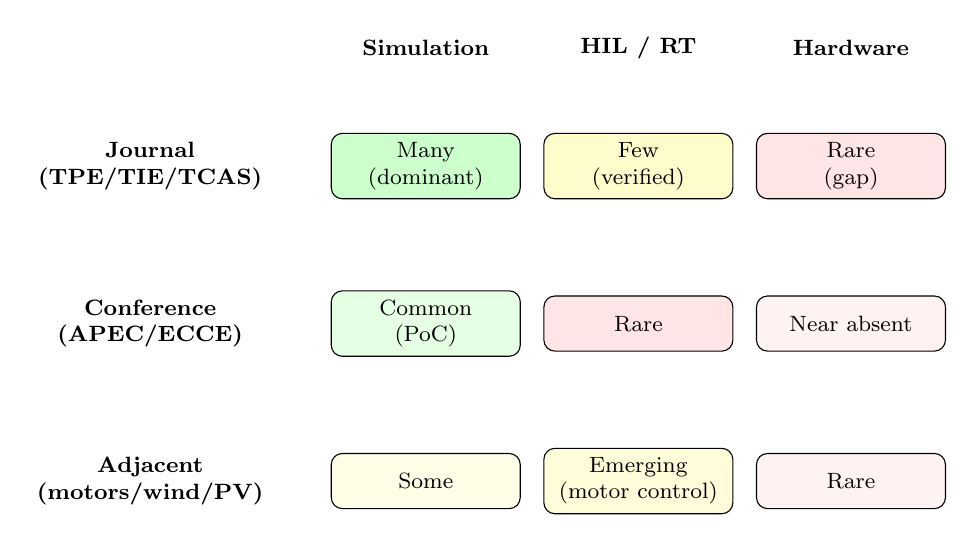
\begin{tikzpicture}[
  node distance=1.5cm,
  box/.style={draw, rounded corners, minimum width=2.4cm, minimum height=0.7cm, align=center, font=\footnotesize},
  rowlabel/.style={font=\footnotesize\bfseries, minimum width=2.0cm, align=center},
  collabel/.style={font=\footnotesize\bfseries, minimum width=2.4cm, align=center}
]

% Column headers
\node[collabel] (c1) at (3.5, 1.0) {Simulation};
\node[collabel] (c2) at (6.2, 1.0) {HIL / RT};
\node[collabel] (c3) at (8.9, 1.0) {Hardware};

% Row labels
\node[rowlabel] (r1) at (0, -0.5) {Journal\\(TPE/TIE/TCAS)};
\node[rowlabel] (r2) at (0, -2.5) {Conference\\(APEC/ECCE)};
\node[rowlabel] (r3) at (0, -4.5) {Adjacent\\(motors/wind/PV)};

% Journal row
\node[box, fill=green!20] (j-sim) at (3.5, -0.5) {Many\\(dominant)};
\node[box, fill=yellow!20] (j-hil) at (6.2, -0.5) {Few\\(verified)};
\node[box, fill=red!10] (j-hw) at (8.9, -0.5) {Rare\\(gap)};

% Conference row
\node[box, fill=green!10] (c-sim) at (3.5, -2.5) {Common\\(PoC)};
\node[box, fill=red!10] (c-hil) at (6.2, -2.5) {Rare};
\node[box, fill=red!5] (c-hw) at (8.9, -2.5) {Near absent};

% Adjacent row
\node[box, fill=yellow!10] (a-sim) at (3.5, -4.5) {Some};
\node[box, fill=yellow!15] (a-hil) at (6.2, -4.5) {Emerging\\(motor control)};
\node[box, fill=red!5] (a-hw) at (8.9, -4.5) {Rare};

% Grid lines (implicit via positioning)

\end{tikzpicture}
\caption{Evidence maturity map summarizing the distribution of validation evidence across venue tiers and validation maturity levels. Green cells indicate well-populated regions; yellow cells indicate emerging but thin evidence; red cells indicate near-absent evidence where more work is needed. The map highlights two structural gaps: the scarcity of hardware-validated (Level~5/6) evidence in preferred-core journals, and the near-absence of HIL or hardware validation in conference proceedings. Adjacent-domain sources (motor drives, wind, PV) provide transferable concepts but are not counted in the converter-control evidence base.}
\label{fig:evidence-maturity-map}
\end{figure}

\subsection{Cross-Axis Synthesis Maps}

Although a full statistical cross-axis map is premature given the current evidence-base coverage, qualitative patterns emerge when the verified sources are placed on the six taxonomy axes simultaneously:

\textbf{Control role vs.\ deployment maturity.}
The verified sources show a clear correlation: hybrid-control roles (coefficient tuning, nonlinear compensation) achieve higher validation maturity (HIL and real-time testbed) than direct-control roles, which remain predominantly at the simulation level.
This pattern is consistent with the engineering intuition that hybrid architectures are easier to validate because the classical controller provides a safety baseline.

\textbf{Algorithm family vs.\ action interface.}
Among the verified sources, continuous-action algorithms (PPO, TD3, DDPG) are used for continuous action interfaces (MFSMC coefficients, MPC coefficients, compensation signals), which is expected since these algorithms are designed for continuous control.
There is no verified evidence of a discrete-action algorithm (DQN) deployed on a continuous action interface through discretization---a design choice that would introduce a resolution tradeoff.

\textbf{Safety mechanism vs.\ deployment readiness.}
The robust-control-wrapper pattern (Level~2 safety) appears in the two sources with the highest deployment maturity: Gheisarnejad Chirani et al.~\cite{gheisarnejad2022reducing} (OPAL-RT HIL) and Meng et al.~\cite{meng2022novel} (experimental validation).
This suggests a virtuous cycle: using a classical controller as a safety wrapper enables more ambitious validation, which in turn produces stronger evidence for the hybrid architecture's deployability.

\textbf{Computation stage vs.\ hardware evidence.}
The only verified source with online adaptation on a real-time platform is Hajihosseini et al.~\cite{hajihosseini2020dc}.
All other verified sources report offline training with online inference only.
This finding underscores a significant gap: evidence-based claims about the feasibility, cost, or safety of online DRL adaptation on embedded converter-control hardware cannot currently be made, because only one verified source reports such evidence, and its computational details are not fully documented in the accessible metadata.

\begin{table}[t]
\caption{Qualitative cross-axis synthesis: verified sources and Tang et al.\ mapped to multiple taxonomy axes. The table complements the prose observations above and highlights where evidence is concentrated and where it is absent.}
\label{tab:cross-axis-synthesis}
\small
\begin{tabular}{p{2.4cm}p{1.8cm}p{1.5cm}p{1.5cm}p{1.5cm}p{1.5cm}}
\toprule
Source & Control role & Algorithm & Safety level & Valid. maturity & Comp. stage \\
\midrule
Hajihosseini et al.~\cite{hajihosseini2020dc} & Hybrid: ULM gain adapt. & Actor-critic & Level~2 (robust wrapper) & Level~4 (real-time embedded) & Offline + online adapt. \\
Meng et al.~\cite{meng2022novel} & Hybrid: nonlinear comp. & TD3 & Level~2 (backstepping baseline) & Exp. validation & Offline train / online infer. \\
Gheisarnejad et al.~\cite{gheisarnejad2022reducing} & Hybrid: coef. tuning & PPO & Level~2 (SMC baseline) & Level~3 (C-HIL, OPAL-RT) & Offline train / online infer. \\
Khooban~\cite{khooban2022smartenance} & Hybrid: MPC coef. design & DDPG & Level~1 (constrained action) & Exp. comparison & Offline train / online infer. \\
Fathollahi et al.~\cite{fathollahi2023robust} & Hybrid: param. tuning (cond.) & SAC (cond.) & Level~1 (reward penalty) & HIL claim (cond.) & Offline train / online infer. \\
Tang et al.~\cite{tang2020reinforcement,tang2021deep,tang2022deep} & Direct: mod. opt. & Q-learning / DDPG / TD3 & Level~0--1 & Level~1 (simulation) & Offline train / online infer. \\
\midrule
Gheisarnejad \& Khooban~\cite{gheisarnejad2020iot} & Hybrid: ADRC tuning & DDPG & Level~1 & Level~4 (real-time impl.) & Offline train / online infer. \\
\bottomrule
\end{tabular}
\end{table}

\subsection{Why the Old Distribution and Timeline Approach Failed}

The prior broad-scope review attempted to present an algorithm-distribution bar chart and a timeline of ``Value-Based Learning (2015--2017), Policy Gradient (2018--2020), Actor-Critic (2021--2023).''
The classification audit (documented separately) revealed that this approach failed along multiple dimensions:

\begin{itemize}
  \item Algorithm labels were inferred from secondary sources, titles, or related-work sections rather than verified from method sections, producing misclassifications (DQN vs.\ DDQN vs.\ Q-learning; TD3 vs.\ DDPG; SAC vs.\ DDPG/Q-learning).
  \item The timeline conflated the year of the original AI/RL algorithm publication with the year of the first PEC adoption and the validation maturity at adoption, obscuring the fact that many ``recent'' PEC papers use algorithms published 3--5 years earlier.
  \item Converter-type aggregation lumped together direct control, hybrid control, and unrelated papers (e.g., maintenance/PHM) under the same heading, producing apparent statistics that were not interpretable.
\end{itemize}

Paper A's response is not to produce a corrected version of the same figures, but to replace them with evidence-gated synthesis maps and qualitative cross-axis observations.
If and when the evidence base is sufficiently verified, a cross-axis deployment-readiness map (control role $\times$ safety mechanism $\times$ deployment maturity) would be the appropriate figure, not an algorithm-distribution bar chart.

%=====================================================================
\section{Open Benchmarks and Reproducibility}
\label{sec:benchmarks}
%=====================================================================

The current DRL-for-converter-control literature is difficult to compare, reproduce, or build upon.
Two papers that both claim ``PPO-based voltage regulation of a buck converter with CPL'' may use different converter parameters (switching frequency, inductance, capacitance), different load-step profiles, different reward functions, different training budgets, and different baseline controllers.
Without standardized reporting, the community cannot determine whether a reported improvement is due to a better algorithm, a more favorable simulator configuration, or more extensive hyperparameter tuning.

This section proposes minimum reporting metadata for reproducible DRL converter-control studies, describes the current state of benchmark availability, and explains why open benchmarks are a prerequisite for moving the field from isolated demonstrations to cumulative progress.

\subsection{Minimum Reporting Metadata}

Table~\ref{tab:reproducibility-checklist} specifies the six categories of information that every DRL converter-control paper should report.
These categories are designed to enable three specific reuse scenarios: (1) a researcher attempting to reproduce the reported results, (2) a researcher comparing a new method against the reported baseline, and (3) a reviewer or survey author classifying the paper for a meta-analysis.

\begin{table*}[t]
\caption{Minimum reporting checklist for reproducible DRL converter-control studies. Paper A will use this checklist both as a benchmark proposal and as a coding schema for future evidence extraction.}
\label{tab:reproducibility-checklist}
\begin{tabular}{p{0.18\textwidth}p{0.34\textwidth}p{0.38\textwidth}}
\toprule
Reporting item & Required details & Purpose in this survey \\
\midrule
Plant and converter model & Converter topology, operating mode, parasitics, load model, grid or source interface, sampling period & Determines whether results transfer across converter families or only hold for a narrow simulation setting. \\
MDP/POMDP definition & State vector, action interface, reward terms, constraints, termination conditions, disturbance process & Enables algorithm comparison without guessing what the learned agent actually observes and controls. \\
Training protocol & Simulator fidelity, episode length, randomization range, baseline initialization, training budget, hyperparameter search & Separates algorithm merit from simulator design, reward engineering, and tuning effort. \\
Safety and stability evidence & Constraint handling, Lyapunov/barrier argument, robust wrapper, shielding logic, stress-test cases, fallback controller & Indicates whether safety is only empirical or supported by an explicit assurance mechanism. \\
Deployment evidence & Processor or real-time simulator, control-loop frequency, latency, memory, HIL/prototype setup, measurement conditions & Supports deployment-readiness claims and prevents hardware feasibility from being inferred from simulation alone. \\
Reproducibility assets & Code, trained policy, environment, benchmark data, test profiles, ablation settings & Allows the survey to identify reusable benchmarks rather than isolated demonstrations. \\
\bottomrule
\end{tabular}
\end{table*}

The reporting checklist is not merely a set of recommendations for future papers; it also serves as a coding schema for Paper~A's evidence extraction.
For each source that enters the evidence table, the six checklist categories are populated with whatever information the source provides, and gaps are explicitly recorded.
This practice reveals systematic reporting gaps: for example, if no paper in the evidence base reports inference latency on the target hardware, the survey can identify this as a collective gap rather than simply noting that individual papers are incomplete.

\subsection{Current Benchmark Landscape}

The verified literature contains no standardized, openly available benchmark environment for DRL-based converter control.
Each research group develops its own simulation environment (typically MATLAB/Simulink with the Simscape Electrical toolbox, or Python with custom ODE solvers), its own disturbance profiles, and its own evaluation metrics.
The closest approximations to reusable environments are:

\begin{itemize}
  \item The RL environment toolbox for electric motor control by Traue et al.~\cite{traue2020toward} (adjacent domain: electric motor drives), which provides a Gym-style interface for motor-control RL tasks. While adjacent (motor drives rather than DC--DC converters), it demonstrates the feasibility and value of standardized RL environments for power-electronic control.
  \item The PLECS RT Box and OPAL-RT platforms, which provide real-time simulation capabilities that can serve as a common hardware-in-the-loop validation target, though they require proprietary hardware and software.
\end{itemize}

In the broader RL community, reproducibility has received systematic attention through initiatives such as the NeurIPS reproducibility program~\cite{pineau2021improving}, open-source reliable implementations such as Stable-Baselines3~\cite{raffin2021stable}, and surveys of benchmarking frameworks~\cite{stapelberg2020survey}.
Henderson et al.~\cite{henderson2018deep} demonstrated that reported performance in DRL can be highly sensitive to hyperparameter choices, random seeds, and implementation details---a finding that applies with particular force to converter-control studies where the simulator configuration is rarely standardized.
These insights are directly relevant to the DRL-for-converter-control community: without shared benchmarks and rigorous reporting standards, the comparison of methods across papers is unreliable.

Several research groups have released code for their specific experiments, but these code releases are typically tied to a single paper, a single converter topology, and a single simulator version, making them difficult to reuse for comparison studies without substantial modification.

\subsection{Why Reproducibility Matters for a CSUR Survey}

A computing survey is not merely a literature review; it is a synthesis that should enable the community to identify what works, what does not, and why.
Without reproducible benchmarks, the survey cannot perform this synthesis beyond qualitative observations.
Concretely, if Paper A states that ``PPO with robust-control wrapping achieves better sim-to-real transfer than DDPG with reward-only safety on buck-converter CPL stabilization,'' this statement requires that (a) the two approaches have been evaluated on comparable tasks, (b) the evaluation metrics are consistent, and (c) the comparison controls for differences in training budget, hyperparameter tuning, and simulator fidelity.
None of these conditions currently holds for the converter-control DRL literature.

Paper~A therefore calls for the development of one or more open benchmark suites that include:
\begin{itemize}
  \item Standardized converter models (buck, boost, DAB, and interleaved boost as a minimum starting set) with well-documented parameters.
  \item A library of disturbance profiles (load steps, input-voltage sags, parameter variations) that span typical and worst-case conditions.
  \item Reference implementations of classical controllers (PI, Type-III, MPC, SMC) as baselines.
  \item Standardized metrics: steady-state voltage regulation error, transient overshoot and settling time, constraint violation rate, inference latency, and training budget.
  \item A reporting template that captures the items in Table~\ref{tab:reproducibility-checklist}.
\end{itemize}
The benchmark suite itself is a computing contribution---a software infrastructure problem that the CSUR readership is well-positioned to address.

%=====================================================================
\section{Research Agenda}
\label{sec:agenda}
%=====================================================================

The preceding synthesis reveals not a mature field approaching saturation, but a field at an inflection point: the number of simulation demonstrations is growing rapidly, but the translation of those demonstrations into deployable, safety-aware, and computationally characterized controllers is lagging.
This section proposes a research agenda structured around five directions, each specifying a current bottleneck, a candidate computing method, a validation metric, and a concrete deployment scenario.
The agenda is summarized in Table~\ref{tab:research-agenda}.

\begin{table*}[t]
\caption{CSUR-oriented research agenda for DRL-based real-time converter control. Each direction is framed as a computing problem with an explicit validation path.}
\label{tab:research-agenda}
\begin{tabular}{p{0.21\textwidth}p{0.25\textwidth}p{0.22\textwidth}p{0.22\textwidth}}
\toprule
Bottleneck & Candidate computing method & Validation metric & Deployment scenario \\
\midrule
Policies trained in narrow simulations fail under unmodeled load, source, and parameter shifts & Domain randomization, uncertainty-aware RL, system-identification loops, and policy adaptation with fallback control & Worst-case voltage/current deviation, recovery time, constraint-violation rate, and transfer success over unseen profiles & Buck/boost/DAB converters feeding CPLs under abrupt load and input-voltage disturbances. \\
Safety claims are often encoded only as reward penalties & Constrained RL, control-barrier functions, Lyapunov-guided critics, runtime shielding, and robust-control wrappers & Constraint satisfaction under transients, safe-set invariance, switching-stress limits, and certified region of operation & Grid-interface converters, onboard DC systems, and microgrid converters with strict current and voltage envelopes. \\
Real-time feasibility is obscured by offline training cost and missing embedded metrics & Policy compression, tiny actor networks, quantization, event-triggered inference, and hardware-aware neural architecture search & Inference latency, memory footprint, processor utilization, sampling-period margin, and adaptation cost & DSP/FPGA/MCU implementation for sub-millisecond converter-control loops. \\
Single-agent demonstrations do not scale to converter-dense networks & Multi-agent RL with communication constraints, graph-based coordination, decentralized critics, and mean-field approximations & Scalability with converter count, communication overhead, stability under packet loss, and fairness of power sharing & Modular converters, ISOP-DAB systems, DC solid-state transformers, and converter-dense microgrids. \\
Results are difficult to compare because environments and reporting conventions differ & Open benchmark environments, standardized disturbance suites, reference controllers, and reproducibility packages & Cross-paper comparability, ablation completeness, repeatability of trained policies, and public artifact availability & Shared CSUR evidence package for converter-control studies across simulation, HIL, and prototype levels. \\
\bottomrule
\end{tabular}
\end{table*}

\subsection{Safety-Guaranteed Learning}

\textbf{Bottleneck.} Current safety mechanisms are almost exclusively reward-level penalties (Level~0) or constrained action sets (Level~1).
Certifiable safety mechanisms---Lyapunov-constrained RL, CBF-based action filtering, formally verified policy properties---have been demonstrated in the theoretical safe-RL literature but not integrated with the power-electronics-specific constraints of switching converters (shoot-through prevention, magnetic saturation, thermal limits, EMI compliance).

\textbf{Candidate computing method.}
Lyapunov-guided critic training uses the known converter dynamics (averaged model) to define a Lyapunov function candidate, and constrains the critic update to respect the Lyapunov decrease condition.
CBF-based action filtering projects the policy's proposed action onto the safe set defined by a control barrier function, using a quadratic program that can be solved in microseconds if the CBF is simple (e.g., a linear function of the inductor current and output voltage).
Runtime shielding with a simplified plant model can filter unsafe actions at the switching frequency.

\textbf{Validation metric.}
Constraint violation rate (number of constraint violations per hour of operation), worst-case transient voltage/current deviation, certified safe-action ratio (fraction of policy outputs that pass shield verification), and Lyapunov-function decrease rate during transients.

\textbf{Deployment scenario.}
Buck and boost converters feeding CPLs, where the negative incremental impedance creates a large-signal instability that is well-understood analytically; DAB converters with transformer saturation constraints; grid-tied inverters with strict current-harmonic limits.

\subsection{Reproducible Benchmarks}

\textbf{Bottleneck.}
The absence of standardized environments, disturbance suites, and reporting conventions prevents cross-paper comparison and cumulative progress.
Each paper evaluates its method on a custom simulator configuration with custom metrics, making it impossible to determine whether an improvement is algorithmic or environmental.

\textbf{Candidate computing method.}
A Gym-style (or Gymnasium-compatible) environment suite for power electronic converter control, providing standardized state, action, and reward interfaces for common converter topologies.
The environment should support multiple simulator backends (Python/ODE, Simulink co-simulation, PLECS co-simulation) and multiple validation levels (offline simulation, real-time simulation, HIL interface).
Reference implementations of classical controllers (PI, Type-III, MPC, SMC) and baseline DRL algorithms (DQN, DDPG, TD3, SAC, PPO) should be included.

\textbf{Validation metric.}
Cross-paper comparability (two papers evaluating on the same benchmark should produce directly comparable metrics), ablation completeness (does the paper report the contribution of each component?), repeatability of trained policies, and public artifact availability (are the code, trained model, environment, and test profiles publicly accessible?).

\textbf{Deployment scenario.}
The benchmark suite itself is the deployment artifact.
It should be released as an open-source repository with documentation, example scripts, and a leaderboard structure similar to established RL benchmarks (OpenAI Gym, DeepMind Control Suite).

\subsection{Hardware-Aware Policies}

\textbf{Bottleneck.}
The gap between a floating-point PyTorch policy running on a GPU workstation and a fixed-point or quantized policy running on a DSP or FPGA is large and poorly characterized.
Without explicit latency, memory, and precision measurements, claims of ``real-time feasibility'' are unsupported.

\textbf{Candidate computing method.}
Policy compression (pruning, quantization, distillation), hardware-aware neural architecture search (NAS) that optimizes for a latency-memory-accuracy Pareto frontier on the target platform, and event-triggered inference that reduces the average computational load.
Tiny actor networks (2--3 hidden layers with 16--64 neurons each, using ReLU or tanh activations) should be evaluated alongside larger networks to establish the performance-efficiency tradeoff.

\textbf{Validation metric.}
Inference latency (mean, maximum, and 99th percentile) measured on the target hardware, memory footprint (ROM for weights, RAM for activations and buffers), processor utilization (percentage of the control period consumed by DRL inference), and performance degradation relative to the floating-point baseline.

\textbf{Deployment scenario.}
DSP (e.g., TI C2000 series) and FPGA (e.g., Xilinx Zynq) implementations for sub-millisecond converter-control loops, with a target inference latency of <10\% of the switching period.

\subsection{Multi-Agent Coordination Under Communication Constraints}

\textbf{Bottleneck.}
Current multi-agent DRL for converter control assumes idealized communication (zero delay, no packet loss, global observability during centralized training).
Real converter-dense systems operate under constrained communication, and the degradation of coordination performance under realistic communication models is not well-characterized.

\textbf{Candidate computing method.}
Communication-aware CTDE where the centralized critic is trained with simulated communication delay and dropout, so that the decentralized actors learn robust coordination policies.
Graph-based critic architectures that exploit the known connectivity topology of converter modules.
Federated RL with differential privacy for settings where converter modules belong to different stakeholders and cannot share raw state data.

\textbf{Validation metric.}
Scalability with converter count (voltage regulation and current-sharing error as functions of the number of modules), communication overhead (bandwidth required per agent), stability under packet loss (coordination error vs.\ packet loss rate), and fairness of power sharing.

\textbf{Deployment scenario.}
ISOP-DAB systems with 4--10 modules, DC SSTs with multi-stage coordination, and DC microgrids with 10--50 converter interfaces.

\subsection{Hybrid Model-Based and Learning-Based Control}

\textbf{Bottleneck.}
The literature largely treats model-based and learning-based control as alternatives rather than as complementary tools.
Power-electronics domain knowledge (averaged models, small-signal transfer functions, large-signal Lyapunov functions) is underutilized in DRL formulations.

\textbf{Candidate computing method.}
Model-informed RL that initializes the policy network to mimic a classical controller (behavior cloning from a PI or MPC controller), then fine-tunes with RL to improve performance beyond the classical baseline.
Uncertainty-aware RL that uses the known converter model for nominal predictions and learns only the residual dynamics (parasitics, aging, load uncertainty).
Grey-box system identification that estimates time-varying parameters (inductance, capacitance, ESR) and provides them as additional state inputs to the DRL policy.

\textbf{Validation metric.}
Performance improvement over the classical baseline (not just over an untrained or random policy), sample efficiency (environment steps to convergence), and robustness to parameter drift (performance retention over a range of inductance, capacitance, and ESR values).

\textbf{Deployment scenario.}
Buck and boost converters with wide-range operation, where a single PI controller cannot be tuned for all operating points; DAB converters with aging magnetics and capacitors.

%=====================================================================
\section{Conclusion}
\label{sec:conclusion}
%=====================================================================

This survey has reframed DRL-based control of power electronic and energy conversion systems as a computing problem in real-time, safety-aware, hardware-constrained, and coordinated decision-making.
The central claim---that a computing-oriented taxonomy reveals deployment-critical information that a converter-type or algorithm-type catalogue obscures---is supported by four findings from the verified evidence base.

First, \textbf{hybrid control architectures dominate verified deployment evidence.}
Every verified source that reports hardware-in-the-loop or real-time testbed validation places DRL in an assistive role: tuning controller coefficients, compensating nonlinear disturbances, or adapting feedback gains, rather than directly actuating power switches.
This pattern is unlikely to be accidental; it reflects an implicit community consensus that embedding DRL inside a classical control structure provides a safety baseline that enables more ambitious validation.

Second, \textbf{safety mechanisms beyond reward penalties are rare.}
The overwhelming majority of papers rely on reward shaping alone, which is not a sufficient safety mechanism for deployment.
Robust-control wrappers, as demonstrated by PPO-assisted MFSMC~\cite{gheisarnejad2022reducing} and TD3-assisted backstepping~\cite{meng2022novel}, represent the current frontier of verified safety assurance.
Certifiable mechanisms---Lyapunov-constrained critics, CBF-based action filtering, formally verified policy properties---remain aspirational for converter control.

Third, \textbf{computational characterization is almost entirely absent from the verified literature.}
Only one verified source~\cite{hajihosseini2020dc} reports online adaptation on a real-time platform, and even that source does not provide explicit inference latency, memory footprint, or processor utilization measurements in the accessible metadata.
The computing systems community cannot evaluate the embedded feasibility of DRL converter controllers without these measurements.

Fourth, \textbf{the absence of open benchmarks is a structural barrier to cumulative progress.}
Without standardized environments, disturbance suites, and reporting conventions, the literature will continue to produce isolated demonstrations rather than comparable results.
A CSUR audience is uniquely positioned to address this gap by contributing benchmark infrastructure---a software engineering and computing-systems problem that requires expertise in reproducible RL, real-time simulation, and embedded systems.

\subsection{Limitations}

This survey has several limitations that should be transparently acknowledged.
The evidence base is deliberately conservative: sources are excluded or marked as conditional unless their method and validation details can be verified from accessible metadata or full-text sources.
This conservatism favors reliability over coverage, but it means that the survey may undercount relevant work whose verification is blocked by paywalls or incomplete metadata.
The current evidence base is weighted toward preferred-core venues (TPE, TIE, TCAS-I/II), which may under-represent contributions from adjacent fields (control theory, robotics, and general machine learning) that are published in venues outside the preferred tier.
The classification of hybrid control roles requires judgment about the boundary between ``DRL tunes the controller'' and ``DRL is the controller''; different readers may draw this boundary differently, and the survey's classifications should be treated as revisable as more source-level evidence becomes available.

\subsection{Outlook}

The gap between the promise of DRL for converter control and the reality of deployable learned controllers is, at present, large.
Closing this gap requires progress on multiple fronts simultaneously: certifiable safety mechanisms that are compatible with microsecond-timescale switching constraints, hardware-aware policy design that targets specific embedded platforms with measured latency and memory budgets, multi-agent coordination algorithms that are robust to realistic communication models, and open benchmark infrastructure that enables the community to compare methods on equal footing.
These are computing problems, not power-electronics problems, and they demand the attention of the computing systems community alongside the power-electronics community that has driven the field to its current state.

The near-term path forward is hybrid: DRL components embedded inside classical control structures, validated on real-time hardware with explicit safety fallbacks, and characterized by measured---not inferred---computational cost.
The long-term vision is learned controllers that match or exceed the performance of model-based designs while providing comparable or superior safety guarantees, running efficiently on embedded hardware, and coordinating seamlessly across converter-dense cyber-physical energy systems.
This survey provides the taxonomy, the evidence-audit methodology, and the research agenda to guide that transition.

\bibliographystyle{ACM-Reference-Format}
\bibliography{paper_a_control_deployment}

\end{document}
